% !TeX program = xelatex
% =============================================================================
%  《随机过程》大作业 —— 两版共用正文（个人版 paper_solo.tex / 团队版 paper_team.tex）
%  题目：学习效率层级演化的随机过程建模与策略推荐
%         ——对一篇 context-dependent DEA 论文的解析、复现与方法替换
%  说明：正文、图表、公式完全一致，两版差别只在封面署名与页眉署名。
%  编译：xelatex paper_solo.tex 或 xelatex paper_team.tex（编译两遍）
% =============================================================================
\documentclass[12pt,a4paper]{ctexart}

\usepackage{geometry}
\geometry{a4paper, top=2.54cm, bottom=2.54cm, left=3.17cm, right=3.17cm,
          headheight=0.5cm, headsep=0.6cm, footskip=1.0cm}

\usepackage{amsmath,amssymb,amsthm,bm}
\usepackage{booktabs,tabularx,multirow,array,longtable}
\usepackage{graphicx}
\usepackage{float}
\usepackage{caption}
\usepackage{enumitem}
\usepackage{xcolor}
\usepackage{fancyhdr}
\usepackage[hidelinks]{hyperref}

\captionsetup{font=small,labelsep=quad}
\captionsetup[table]{position=top,skip=4pt}
\captionsetup[figure]{position=bottom,skip=4pt}
\graphicspath{{fig/}}

% ---- 版式：正文小四(12pt)，1.5 倍行距，首行缩进 2 字符 -------------------
\linespread{1.5}
\setlength{\parindent}{2em}
\setlength{\parskip}{0pt}

% ---- 两版差异：封面与页眉的署名 ------------------------------------------
\ifdefined\teamversion
  \newcommand{\authortag}{吴桐\quad 赵睿\quad 张文琦\quad 吴梦豪}
  \newcommand{\coverfile}{tex/00_cover_team}
\else
  \newcommand{\authortag}{吴桐}
  \newcommand{\coverfile}{tex/00_cover_solo}
\fi

% ---- 页眉：左标题、右署名，页脚居中页码 ----------------------------------
\pagestyle{fancy}
\fancyhf{}
\fancyhead[L]{\zihao{-5}\heiti 学习效率层级演化的随机过程建模与策略推荐}
\fancyhead[R]{\zihao{-5}\heiti \authortag}
\fancyfoot[C]{\zihao{-5}\thepage}
\renewcommand{\headrulewidth}{0.4pt}
\renewcommand{\footrulewidth}{0pt}

% ---- 标题格式：一级标题黑体加粗12pt左对齐，中文数字编号 ------------------
\ctexset{
  section = {
    name    = {,、},
    number  = \chinese{section},
    format  = \heiti\bfseries\fontsize{12pt}{20pt}\selectfont\raggedright,
    beforeskip = 14pt plus 3pt minus 2pt,
    afterskip  = 8pt plus 2pt,
  },
  subsection = {
    name    = {（,）},
    number  = \chinese{subsection},
    format  = \heiti\bfseries\fontsize{12pt}{18pt}\selectfont\raggedright,
    beforeskip = 10pt plus 2pt minus 1pt,
    afterskip  = 6pt plus 1pt,
  },
  subsubsection = {
    name    = {,.},
    number  = \arabic{subsubsection},
    aftername = \quad,
    format  = \heiti\bfseries\fontsize{12pt}{18pt}\selectfont\raggedright,
    beforeskip = 8pt plus 2pt minus 1pt,
    afterskip  = 4pt plus 1pt,
  },
}

% ---- 定理类环境 -----------------------------------------------------------
\theoremstyle{definition}
\newtheorem{definition}{定义}[subsection]
\newtheorem{proposition}{命题}[subsection]
\newtheorem{remark}{注}[subsection]
\renewcommand{\proofname}{\heiti 证明}

% ---- 常用记号 -------------------------------------------------------------
\newcommand{\E}{\mathbb{E}}
\newcommand{\Var}{\operatorname{Var}}
\newcommand{\Pbb}{\mathbb{P}}
\newcommand{\R}{\mathbb{R}}
\newcommand{\dd}{\,\mathrm{d}}
\newcommand{\ii}{\mathrm{i}}
\newcommand{\bx}{\bm{x}}
\newcommand{\bz}{\bm{z}}
\newcommand{\bdelta}{\bm{\delta}}
\newcommand{\btheta}{\bm{\theta}}
\newcommand{\bpi}{\bm{\pi}}
\newcommand{\bQ}{\bm{Q}}
\newcommand{\bP}{\bm{P}}
\newcommand{\bA}{\bm{A}}
\newcommand{\bL}{\bm{L}}
\newcommand{\bX}{\bm{X}}
\newcommand{\bY}{\bm{Y}}
\newcommand{\bZ}{\bm{Z}}
\newcommand{\refs}[1]{$^{[#1]}$}

% 表格通用：五号字
\newcommand{\tabfont}{\zihao{5}\selectfont}

\begin{document}

\input{\coverfile}
% =============================================================================
%  摘要与关键词
% =============================================================================
\begin{center}
{\heiti\bfseries\fontsize{14pt}{22pt}\selectfont 摘\quad 要}
\end{center}

\vspace{0.2cm}

本文以一篇基于 context-dependent DEA 的学习策略推荐论文（Expert Systems
with Applications, 2023）为对象，完成解析、复现与方法替换三项工作。首先把
原文“复合量化—聚类—类内 DEA—分层—三准则—参考路径”的证据链还原为可检验
的数学表述，指出层级不可跨群体迁移、参考路径本质是对高效同伴的模仿、障碍
度公式与表中数值不自洽等结构性局限。其次在不掌握原始问卷的条件下，依据题
项分布与锚点约束逆向重建 519 份样本，用 R 实现 PAM-Gower 聚类、类内
CCR-DEA 与分层，复现出同构的五类结构以及个体 S480 单步 26.31\%、累计
47.69\% 的提升路径。最后以随机过程替换静态评价：把五级效率层级视为状态空
间，建立带协变量的生灭过程并作极大似然估计，解析求解首达时间并用 Gillespie
模拟校验，再以 Ornstein-Uhlenbeck 扩散刻画连续效率，在学时预算下求解最优
策略。所用工具限于 Poisson 过程与一致化、Markov 链的极限定理与谱隙、鞅的停时
定理、Brown 运动的反射原理与反正弦律、Itô 公式，不涉及更新过程。
16 周末已不在第 5 层的概率 0.642、期望效率提升 25.53\% 与原文 25.38\% 相互印证；模型
还给出了原文缺失的时间尺度（中位 14.5 周，累计 43.97\% 需 53.7 周）、“增加
投入反而降低 DEA 效率”的机制性解释，以及两个只靠截面数据即可成立的结论：
从第 4 层出发先跌回第 5 层的概率为 86\%，仅靠自然波动在 16 周内触及 0.95 的
机会不足 1.5\%。

\vspace{0.4cm}

\noindent{\heiti 关键词：}随机过程；生灭过程；首达时间；数据包络分析；
context-dependent DEA；学习策略推荐


\newpage
\tableofcontents
\newpage

% =============================================================================
%  一、问题陈述
% =============================================================================
\section{问题陈述}

\subsection{研究背景：从“投入多少”到“效率多高”}

高等教育的评价对象正在从“教得好不好”扩展到“学得会不会”。随着学分制与自
主学习的推行，同一门课程里学生可自由支配的课外时间显著增加，学习结果却呈
现出很大的离散性：有人每天投入四五个小时却收效有限，有人在较短时间内完成
听说读写的闭环并取得高分。教育心理学把这种差异归因于学习策略，即学生在时
间分配、复习方式、应试训练、心理调适与兴趣拓展上的组合选择。于是，教学管
理者真正关心的问题并不是“谁更努力”，而是“在给定的投入组合下，谁的转化效
率更高；效率低的人应当朝哪个方向、以多大强度调整，才能以可接受的时间代价
上一个台阶”。

传统上回答这一问题依靠三类工具：其一是相关分析与回归，它给出“某行为与成
绩同向变动”的平均结论，却无法处理多投入、多产出之间的替代关系；其二是问
卷描述统计，它告诉我们学生“做了什么”，不回答“做得值不值”；其三是聚类或
潜类分析，它把学生分成若干类型，但类型本身没有优劣，无法直接转化为建议。
数据包络分析（Data Envelopment Analysis, DEA）\refs{1} 的引入改变了这一点：
它把每个学生视为一个决策单元（Decision Making Unit, DMU），用线性规划在
“投入—产出”空间中构造前沿面，把个体的相对效率写成投入可压缩的比例，从而
在同一标尺下比较“转化能力”。这一思路在教育效率、学校绩效与资源配置中被广
泛使用。

然而，标准 DEA 只回答“你现在离前沿有多远”，不回答“你离前沿远是因为起点
差，还是因为路径差”。为区分这两种情形，Seiford 与 Zhu 提出
context-dependent DEA\refs{2}：先剔除强有效单元，再在剩余集合上重新评价，
如此逐层剥离，得到一个由外向内的效率分层结构，并用吸引力、进步度、邻近度
三个指标描述个体在层间的相对位置。这一想法被后续研究用于技术效率的分级、
区域经济梯度与医院绩效的阶梯式改进。

\subsection{被解析的论文及其贡献}

本文解析的对象是 Zhao 等人 2023 年发表于 \textit{Expert Systems with
Applications} 第 211 卷的研究\refs{3}。该文以北京某高校 519 名非英语专业本
科生的英语课程为背景，围绕 14 个学习行为题项（兴趣、复习、考试次数、临场
状态、心理、休息、模拟考、背诵、听力、口语、阅读、课外拓展、辅导、出国意
愿）构造了一个名为 CHPI 的推荐框架，其流程可概括为四个步骤：

\begin{enumerate}[label=（\arabic*）,itemsep=2pt,topsep=2pt,leftmargin=3em]
\item \textbf{复合量化}：不同题项的量纲与题型并不一致（五级有序、计数、连
  续时长），原文用“累积百分比法”把每一题的作答映射为 0—100 的得分，再按题
  型加权合成 4 个投入指标与 1 个产出指标，并以题项方差 $\sigma^2<10$ 作为
  “信息量不足需重赋权”的判据；
\item \textbf{本体聚类}：以 Gower 距离处理混合数据类型，用 PAM
  （$k$-medoids）把学生分为 5 类，理由是“不同学习风格的学生不应放在同一个
  前沿面上比较”；
\item \textbf{类内效率评价}：在每一类内部用投入导向的 CCR 模型计算效率
  $\theta_i$，并用 $\varepsilon$ 松弛与 Archimedes 无穷小处理弱有效；
\item \textbf{分层与路径推荐}：用 context-dependent DEA 的剔除式算法把每类
  再分为 5 层，计算吸引力 $\Omega$、进步度 $P$、邻近度 $D$ 与障碍度 $H$，
  再按“上一层中 $H$ 最小、距离最近”的规则为个体拼接一条逐层上升的参考路
  径。原文以 5 类中的第 5 类、效率 0.6771 的学生 S480 为例，给出
  S480$\to$S502$\to$S216$\to$S18 的四步路径，单步提升 25.38\%，累计提升
  43.97\%。
\end{enumerate}

这篇论文的价值在于把“效率评价”推进到“效率分层”，再把“分层”推进到“个体
路径”，在方法论上完成了从静态打分到结构化建议的跨越；在应用上，它给出了
一套可执行的数据处理口径（尤其是混合题型的统一量化），这对教育数据挖掘领
域具有直接的借鉴意义。也正因为它在这条链条上走得足够远，链条上每一环的薄
弱之处才暴露得格外清楚。

\subsection{原文的三处结构性局限}

\textbf{第一，评价是静态的，缺少时间维度。}原文的效率 $\theta_i$ 是某一学
期截面数据的比值，层级是个体在这一截面中的相对位置。于是它只能回答“谁在
这一层”，不能回答“从这一层到上一层平均需要多久”“这一跃迁的概率有多大”
“跳上去之后能否稳住”。对教学干预而言，这三个问题恰恰是最要紧的：一个需要
八周、成功率六成的建议，与一个需要一年、成功率一成的建议，其优先级完全不
同。

\textbf{第二，层级依赖参照集，不可跨群体迁移。}剔除式分层把“被当前前沿
支配的单元”留在下一层，层数由数据本身的效率分布决定，而不是由某个外生标
准决定。这意味着同一名学生在不同班级、不同学期、不同题项权重下会被分到不
同的层；层级不是一把可以随身携带的尺子，而是一张只对当前样本有效的排名
表。原文把层号直接写进推荐语（“从第 5 层升到第 4 层”），在跨群体使用时缺
少可解释性。

\textbf{第三，推荐机制本质上是“模仿”，而非“最优控制”。}路径规则是在上一
层中找 $H$ 最小、$L_1$ 距离最近的同伴，令个体向其行为组合靠拢。这一规则隐
含两个强假设：其一，同样的行为组合在不同个体身上产生同样的效率（忽略个体
异质性与边际收益递减）；其二，越接近高效同伴就越优（忽略了“投入已经饱和、
再加投入反而稀释效率”的可能）。更实际的问题是，它只告诉学生“跟谁学”，不
告诉学生“学多少、练多久、先做哪一项”。

除这三处结构性局限之外，本文在核对原文表格时还发现一处内部不一致：原文
文字部分把障碍度定义为 $H=1/\Omega+P$，但表 3 中给出的 $H$ 值与同一行的
$(\Omega,P)$ 无法对应。例如某个体 $\Omega=0.0514$、$P=0.0096$，按定义应得
$H\approx 19.5$，而表中 $H=0.43$。这说明原文在指标合成或表格转录环节存在未
披露的处理，也说明“三准则”的可复现性需要逐项检验，而不能照抄公式。

\subsection{本文的任务与组织结构}

基于上述判断，本文把工作拆成三个前后衔接、权重相当的部分，并以“能否被独立
复算”作为唯一的验收标准。

\begin{enumerate}[label=（\arabic*）,itemsep=3pt,topsep=3pt,leftmargin=3em]
\item \textbf{破解}：把原文从“问卷题项”到“推荐路径”的全过程拆成“输入—变
  换—输出”的证据链，逐步写出数学形式、算法伪码与隐含假设，标注每一步的
  自由度（哪些参数由数据决定、哪些由作者选择、哪些未披露），从而回答“这篇
  论文究竟做了什么、凭什么成立”。
\item \textbf{复现}：在拿不到原始问卷的前提下，以题项分布、样本规模、类规
  模、以及原文公开的锚点（S480 的效率 0.6771、单步 25.38\%、累计
  43.97\%）为约束，逆向重建一份可计算的数据集，用 R 语言实现
  PAM-Gower 聚类、类内 CCR-DEA、分层与三准则，逐项与原文对照，并对偏差给
  出机制性解释。
\item \textbf{替换}：不再使用 context-dependent DEA，而用随机过程重建同一
  主题。把五级效率层级视为状态空间，建立带协变量的生灭过程，估计转移强度，
  解析求解首达时间，用 Gillespie 算法校验；再用 Ornstein-Uhlenbeck 扩散刻
  画连续效率的随机演化，最后在学时预算约束下求解“哪几项动作、各投入多少”
  的最优策略。与原文的静态排序相比，这套方法输出的是“概率—时间—策略”的
  三元组。
\end{enumerate}

三部分的技术路线与交付物见表~\ref{tab:route}。需要说明的是，第一、二部分
并非“铺垫”，它们承担两项不可替代的功能：其一，只有把原文的每一步都复算出
来，替换方法时才能保证“数据、主题、评价对象”三者不变，从而使新旧方法的差
异可归因于方法本身；其二，复现过程中暴露的口径问题（层级定义、指标合成、
聚类数选择）正是随机过程建模必须重新回答的问题——例如“状态”究竟应当是剔除
式层级，还是可以保证占满状态空间的分位带层级。

\begin{table}[htbp]
\centering
\tabfont
\caption{本文三阶段任务、方法与交付物}
\label{tab:route}
\begin{tabularx}{\textwidth}{@{}p{1.5cm}p{3.7cm}Xp{3.6cm}@{}}
\toprule
阶段 & 输入 & 主要方法 & 交付物 \\
\midrule
破解 & 原文 PDF（12 页）、
公开表格 & 证据链拆解、公式重述、算法还原、自由度标注 &
  流程图、公式表、可复现性判定表 \\
复现 & 题项分布与锚点约束 &
  累积百分比量化、Gower 距离、PAM、CCR-DEA、分位带与剔除式分层 &
  519 人数据集、效率与层级、锚点对照表、9 幅插图 \\
替换 & 同一数据集、同一主题 &
  生灭过程、极大似然、鞅停时、首达时间、Poisson 一致化、反射原理、Itô 公式、OU 扩散、预算约束优化 &
  转移强度、时间尺度、跃层概率、最优策略、新旧对比表 \\
\bottomrule
\end{tabularx}
\end{table}

全文余下部分安排如下：第二节把实际问题翻译为数学问题，并说明为什么随机过
程是合适的语言；第三节是主体，依次给出原文解析、CHPI 复现、随机过程重构与
系统对比；第四节总结结论、局限与可延伸的方向。


% =============================================================================
%  二、问题分析
% =============================================================================
\section{问题分析}

\subsection{三个映射：从问卷作答到状态轨道}

把一个“学习策略推荐”问题写成数学问题，本质上要连续做三次映射，每一次映射
都会丢失一部分信息，也都需要一次假设来补足。

\textbf{映射一（量化）：作答 $\to$ 投入产出向量。}设第 $i$ 名学生回答了
$p=14$ 个题项，第 $j$ 题的原始作答为 $r_{ij}$。不同题型的取值域不同（五级
有序、0—12 计数、0—20 小时连续），不能直接相加。记量化算子为
$q_j:\mathcal{R}_j\to[0,100]$，则个体被表示为
\begin{equation}
\bx_i=\bigl(x_{i1},x_{i2},x_{i3},x_{i4}\bigr)^{\top}\in\R_+^4,\qquad
y_i\in[0,100],
\label{eq:map1}
\end{equation}
其中 $x_{i1}$ 为听说读背等输入型训练的合成得分，$x_{i2}$ 为考试与模拟考的
训练量，$x_{i3}$ 为复习、辅导与课外拓展的时间投入，$x_{i4}$ 为心理与休息的
调节水平，$y_i$ 为期末成绩。量化算子的选择决定了后续一切结论的尺度，因此它
是复现工作的第一道关口。

\textbf{映射二（评价）：向量 $\to$ 效率。}在给定参照集 $\mathcal{S}$（同一
类学生的集合）下，用投入导向的 CCR 模型把个体映射为一个标量
\begin{equation}
\theta_i=\min\Bigl\{\theta\;\Big|\;\exists\,\bm{\lambda}\ge \bm{0}:\;
\sum_{j\in\mathcal{S}}\lambda_j\bx_j\le\theta\bx_i,\;
\sum_{j\in\mathcal{S}}\lambda_j y_j\ge y_i\Bigr\}\in(0,1].
\label{eq:map2}
\end{equation}
$\theta_i=1$ 表示位于前沿，$\theta_i<1$ 表示在同等产出下投入可压缩的比例。
效率把四维投入压缩成一维比值，代价是丢失了“哪一项投入最冗余”的信息——这
一信息只能从对偶乘子或松弛变量中部分找回。

\textbf{映射三（分层）：效率 $\to$ 层级。}把连续效率离散化为有限个有序等
级，是引入时间维度的前提。原文采用剔除式分层：先取 $\theta=1$ 的强有效单
元为第 1 层并从集合中剔除，在剩余集合上重算效率，再取新出现的 $\theta=1$
单元为第 2 层，如此反复。设第 $k$ 层集合为 $E_k$，则
\begin{equation}
E_1=\bigl\{i:\theta_i^{\mathcal{S}}=1\bigr\},\quad
E_{k}=\Bigl\{i:\theta_i^{\mathcal{S}\setminus\cup_{j<k}E_j}=1\Bigr\},\ k\ge 2 .
\label{eq:map3}
\end{equation}
这一映射有一个不易察觉的性质：层号不是个体的固有属性，而是“相对于当前参照
集的位置”。参照集一变，层号就变。这一点在第二节已作为局限提出，在第三节
将给出另一种口径（类内效率分位带），它把层号变成“同类群体中的百分位”，从
而保证了状态空间的占满性与可比性。

三次映射复合起来，一名学生在一个学期内就对应一条轨道
\begin{equation}
\bigl(r_{i1},\dots,r_{ip}\bigr)\;\longrightarrow\;\bx_i,y_i
\;\longrightarrow\;\theta_i\;\longrightarrow\;S_i\in\{1,\dots,5\}.
\label{eq:track}
\end{equation}
原文止步于 $S_i$，把它当作静态标签；本文则把 $S_i$ 当作随机过程的取值，让
它随学期内的时间演化。

\subsection{静态评价的数学结构与三处缺口}

把 DEA 写成式\eqref{eq:map2} 的形式后，可以清楚地看到它的三个数学特征，这
三个特征正是静态评价的边界。

\textbf{其一，评价是“截面”的。}$\theta_i$ 只依赖于同一时点的
$\{\bx_j,y_j\}_{j\in\mathcal{S}}$，与时间无关。若把 $\theta$ 视为一个随机
变量，DEA 给出的是它的一个实现值，而不是它的分布或演化规律。

\textbf{其二，评价是“相对”的。}$\theta_i$ 的大小取决于参照集的构成：当参
照集中出现一个投入更少、产出更高的个体时，所有人的效率都会下降。这意味着
效率值不可跨群体加总，也不可跨学期直接比较；原文的分层因此只能在样本内部
解释。

\textbf{其三，评价是“无记忆”的。}$\theta_i$ 不携带历史信息：一名学生上一
学期效率是 0.5、本学期是 0.8，与另一名一直稳定在 0.8 的学生，在静态评价中
完全等价。教育干预真正关心的“进步速度”“退步风险”“维持时间”在静态框架中
没有位置。

由此可以列出三处缺口，它们分别对应本文要用随机过程补上的三件事：

\begin{enumerate}[label=（\arabic*）,itemsep=2pt,topsep=2pt,leftmargin=3em]
\item \textbf{无转移概率}：给定当前层级 $k$，下一阶段处于各层级的概率未知。
  补法是把层级序列建成连续时间马尔可夫链，用转移强度矩阵 $\bQ$ 描述“上
  一层”与“下一层”的瞬时速率。
\item \textbf{无时间尺度}：从第 $k$ 层到第 1 层的平均等待时间未知。补法是
  求首达时间的期望 $m_k=\E_k[T_1]$，它满足一个三对角线性方程组，可解析求
  解并用蒙特卡洛校验。
\item \textbf{无策略空间}：原文的“路径”是同伴的复制，不是可优化的决策。补
  法是把行为改变写成动作集 $\mathcal{A}$，在学时预算约束下最大化
  $\E[\theta_T]$ 或最小化 $\E[T_1]$，从而得到“做哪几项、各做多少”的答案。
\end{enumerate}

\subsection{为什么随机过程是合适的语言}

学习效率的演化有三个特征，恰好与随机过程的三类基本对象对应。

\textbf{（1）状态是离散、有序、可反复穿越的。}层级只能取 1—5，且 1 优于 2
优于 $\cdots$ 优于 5；学生可以在相邻层之间来回移动，不能一次跨两层。这与
生灭过程（birth-death process）的状态结构完全一致：状态空间
$\{1,\dots,K\}$，只允许相邻转移，$1$ 与 $K$ 为反射壁。把“上行”记为出生、
“下行”记为死亡，则过程由两列强度刻画：
\begin{equation}
\lambda_k=\lim_{\Delta t\downarrow 0}\frac{\Pbb(S_{t+\Delta t}=k-1\mid S_t=k)}{\Delta t},
\qquad
\mu_k=\lim_{\Delta t\downarrow 0}\frac{\Pbb(S_{t+\Delta t}=k+1\mid S_t=k)}{\Delta t},
\label{eq:rates}
\end{equation}
生成矩阵 $\bQ=(q_{kl})$ 满足 $q_{k,k-1}=\lambda_k$、$q_{k,k+1}=\mu_k$、
$q_{kk}=-(\lambda_k+\mu_k)$。这一结构的最大好处是：平稳分布有闭式解，首达
时间有线性方程组，二者都可以写成可复算的公式，而不是黑箱输出。

\textbf{（2）强度依赖于协变量，个体之间存在系统性差异。}把 $\lambda_k,\mu_k$
写成行为协变量 $\bz_i$ 的函数，可以让“哪一种行为改变最能提高上行强度”成为
可估计的参数问题。这一层对应 Cox 型强度模型与多状态模型的极大似然估计。

\textbf{（3）效率本身是连续的，离散化会损失信息。}层级是粗粒化，真实效率
$\theta_t$ 在 $[0,1]$ 上连续演化，受大量未观测因素（教师风格、教材难度、
同伴影响）驱动。把它写成均值回复的扩散过程
\begin{equation}
\dd\theta_t=\kappa\bigl(\theta^{*}-\theta_t\bigr)\dd t+\sigma\dd W_t,
\qquad \kappa>0,
\label{eq:ou}
\end{equation}
既能刻画“效率有回归均值的天性”，又能给出首达某一目标水平的期望时间闭式
解，从而把“需要多久”的问题从离散链推广到连续时间。

三层结构（离散状态层、强度协变量层、连续扩散层）并非重复，而是分别回答
“在哪一层”“多快能上一层”“连续效率如何波动”。第三节将依次实现这三层。

\subsection{数据可识别性与建模假设}

本文最需要在方法论上说清楚的一点是：\textbf{没有纵向面板数据时，转移强度
不能被单期截面唯一识别。}设观测只有一期的层级 $S_i$，则 $\bQ$ 的
$K(K-1)$ 个参数中，只有平稳分布 $\bpi$ 可被截面频率约束，其余自由度需要
额外信息。本文采用三条互补的信息源来“部分识别”：

\begin{enumerate}[label=（\arabic*）,itemsep=2pt,topsep=2pt,leftmargin=3em]
\item \textbf{协变量差异}：不同学生在复习、应试、输入训练、心理作息与兴趣
  拓展上的差异，使 $\rho_i=\exp(\alpha+\bdelta^{\top}\bz_i)$ 可以被识别到
  相对大小；个体间 $\rho$ 的排序由数据决定，绝对尺度不可识别。
\item \textbf{时间锚点}：以原文给出的“S480 一个学期单步提升 25.38\%”为锚，
  反解时间单位，得到 $c$（每周的总体强度水平）。这是唯一的外部信息，也是
  本文唯一“借来”的参数。
\item \textbf{平稳性约束}：把模型隐含的平稳分布与观测到的层级频率对比，
  用拟合优度检验判断模型是否至少能复现截面结构。
\end{enumerate}

在此框架下，本文明确列出五条建模假设，后续所有结论都以此为前提：

\begin{description}[leftmargin=2em,itemsep=1pt,topsep=2pt]
\item[A1] 层级有序且相邻可达，1 为最优、5 为最差，两端为反射壁；
\item[A2] 在一个学期内，给定协变量后层级演化是时间齐次的马尔可夫链（行为
  习惯的惯性远大于其变化速度）；
\item[A3] 个体之间条件独立，即不存在同伴效应的即时传染（这一条在结论部分
  作为局限讨论）；
\item[A4] 层内效率同质，用层内均值 $\bar\theta_k$ 作为该层的代表效率，用于
  把层级轨道折算为效率轨道；
\item[A5] 行为改变的时间尺度以“周”为单位，一个学期按 16 周计。
\end{description}

\subsection{技术路线与记号约定}

据此，全文的计算路线为：先用原文口径复现 $\theta_i$ 与层级，得到状态序列；
再以状态序列与协变量估计 $\rho_i$ 与 $c$，得到 $\bQ_i$；用 $\bQ_i$ 计算
转移概率、期望效率与首达时间；用 OU 扩散补充连续效率的时间尺度；最后在
动作集上做预算约束优化。为避免符号混淆，本文统一约定：

\begin{itemize}[leftmargin=2em,itemsep=1pt,topsep=2pt]
\item $i=1,\dots,n$ 表示个体，$n=519$；$j$ 表示投入指标，$j=1,\dots,4$；
\item $k,l\in\{1,\dots,5\}$ 表示层级，$k=1$ 为最高效层；
\item $\theta_i$ 为类内 CCR 效率，$S_i$ 为层级，$\bar\theta_k$ 为层均效率；
\item $\Omega_i,P_i,D_i,H_i$ 为原文三准则（吸引力、进步度、邻近度、障碍度）；
\item $\lambda_k,\mu_k$ 为生灭过程的上行、下行强度，$\bQ$ 为生成矩阵，
  $\bP(t)=\exp(\bQ t)$ 为转移概率矩阵；
\item $T_1=\inf\{t:S_t=1\}$ 为首达最高层的时间，$m_k=\E_k[T_1]$。
\end{itemize}

% =============================================================================
%  三、问题求解（一）：原文解析
% =============================================================================
\section{问题求解}

\subsection{原文解析：把论文拆成一条可检验的证据链}

读一篇方法论文，最容易犯的错误是“顺着作者的叙述读”，因为叙述顺序往往按
“动机—方法—结果”组织，而不是按“输入—变换—输出”组织。要判断一篇论文能
不能被复现，必须把它拆成一条链：每一个环节吃进什么、吐出什么、用什么数学
工具完成变换、留下了哪些自由度。按这一标准，原文可拆为五个环节（表
\ref{tab:chain}）。

\begin{table}[htbp]
\centering
\tabfont
\caption{原文的五环证据链及其数学工具}
\label{tab:chain}
\begin{tabularx}{\textwidth}{@{}p{1.0cm}p{2.4cm}Xp{4.3cm}@{}}
\toprule
环节 & 名称 & 变换（输入 $\to$ 输出） & 数学工具 \\
\midrule
1 & 复合量化 & 14 个异质题项的作答 $\to$
  4 维投入 $\bx_i$ 与产出 $y_i$ & 累积百分比法、经验分布函数、
  加权合成 \\
2 & 本体聚类 & $(\bx_i,y_i)$ $\to$ 类别标签 $c_i\in\{1,\dots,5\}$ &
  Gower 距离、PAM（$k$-medoids） \\
3 & 类内评价 & 类内样本 $\to$ 效率 $\theta_i\in(0,1]$ &
  投入导向 CCR-DEA、$\varepsilon$ 松弛 \\
4 & 层级分解 & $\theta_i$ $\to$ 层号 $S_i\in\{1,\dots,5\}$ &
  context-dependent DEA（剔除式） \\
5 & 准则与路径 & 层号 $\to$ 三准则与参考路径 &
  产出导向 DEA、$L_1$ 距离、贪心拼接 \\
\bottomrule
\end{tabularx}
\end{table}

这条链的信息流是单向的：环节 1 的量化口径决定环节 3 的效率，环节 3 的效率
决定环节 4 的层级，环节 4 的层级决定环节 5 的路径。因此\textbf{链上任何一
环的口径变化都会沿着链条放大}。这也是复现工作的难点：即使算法完全正确，只
要量化口径不同，最终的路径就会不同。下面逐环给出数学表述。

\subsubsection{环节 1：复合量化}

设第 $j$ 题有 $K_j$ 个取值档（有序题 $K_j=5$，计数题 $K_j=13$，时长题按
小时离散），第 $k$ 档的样本比例为 $p_{jk}$，累计比例为
$F_{jk}=\sum_{m\le k}p_{jm}$。原文的“累积百分比法”可写成
\begin{equation}
s_{ij}=100\Bigl[1-F_{j,r_{ij}}+\tfrac12 p_{j,r_{ij}}\Bigr],
\label{eq:quant}
\end{equation}
即“优于该档的人数比例”加上“同档人数的一半”，等价于用分位中点作为该档的
代表分位。这样处理的好处是：无论题型如何，得分都落在 $[0,100]$ 且分布近似
均匀，从而消除量纲差异；代价是把原始作答的绝对信息（例如“每天背 3 小时”
与“每天背 4 小时”的差别）压缩成了相对位次。

对计数与时长题，原文改用经验分布函数映射。本文复现时对时长先作
$\log(1+t)$ 变换再取秩，以抑制长尾（少数学生每天投入 8 小时以上会拉开过大
差距）。合成规则为四项投入的组内平均：
\begin{equation}
\begin{aligned}
x_{i1}&=\tfrac14\bigl(s_{\mathrm{rec}}+s_{\mathrm{lis}}+s_{\mathrm{spk}}+s_{\mathrm{rd}}\bigr),\\
x_{i2}&=\tfrac12\bigl(s_{\mathrm{exm}}+s_{\mathrm{mck}}\bigr),\qquad
x_{i3}=\tfrac13\bigl(s_{\mathrm{rev}}+s_{\mathrm{tut}}+s_{\mathrm{ext}}\bigr),\\
x_{i4}&=\tfrac12\bigl(s_{\mathrm{men}}+s_{\mathrm{rst}}\bigr),
\end{aligned}
\label{eq:composite}
\end{equation}
产出 $y_i$ 为期末成绩（0—100）。

原文另设一条“信息量判据”：若某题项的量化得分方差
$\sigma_j^2=\frac1n\sum_i(s_{ij}-\bar s_j)^2<10$，则认为该题区分度不足，
需要重赋权。这一判据在数学上等价于要求标准差大于 3.16 分（百分制），用意
可以理解，但阈值缺乏推导；本文复现时保留该判据作为诊断，并在触发时改用潜
变量秩重映射，以保证该题仍然携带排序信息。

\subsubsection{环节 2：Gower 距离与 PAM 聚类}

14 个题项混合了有序、计数与连续三种类型，欧氏距离不适用。Gower 距离把每
一维的差异归一到 $[0,1]$ 后加权平均\refs{4}：
\begin{equation}
\begin{aligned}
d(i,i')&=\frac{\sum_{j=1}^{p}w_j\,\delta_{j}(i,i')\,d_j(i,i')}
{\sum_{j=1}^{p}w_j\,\delta_j(i,i')},\\
d_j(i,i')&=\frac{|s_{ij}-s_{i'j}|}{\max_{i''}s_{i''j}-\min_{i''}s_{i''j}},
\end{aligned}
\label{eq:gower}
\end{equation}
其中 $\delta_j\in\{0,1\}$ 表示该维是否可比（缺失时取 0）。聚类采用 PAM，
即在小样本下比 $k$-means 更稳健的 $k$-medoids 方法\refs{5}：它不要求均值
存在，直接用“中心点”作为类的代表，最小化
\begin{equation}
W(\mathcal{M})=\sum_{i=1}^{n}\min_{m\in\mathcal{M}}d(i,m),
\qquad \mathcal{M}\subset\{1,\dots,n\},\ |\mathcal{M}|=k .
\label{eq:pam}
\end{equation}
算法上分 BUILD 与 SWAP 两步（算法 1）。

\begin{center}
\fbox{\parbox{0.93\textwidth}{
\tabfont
\textbf{算法 1}\ \ PAM 聚类的 BUILD--SWAP 过程\\[2pt]
\textbf{输入：}距离矩阵 $D=(d(i,i'))$，类数 $k$\\
\textbf{输出：}中心点集合 $\mathcal{M}$ 与标签 $c_i$\\
1.\ BUILD：取使 $\sum_{i'}d(i,i')$ 最小的点为首个中心；\\
2.\ 重复至 $|\mathcal{M}|=k$：取使 $W(\mathcal{M}\cup\{m\})$ 下降最多的未选点加入；\\
3.\ SWAP：对每个 $(m,h)\in\mathcal{M}\times(\mathcal{M}^{c})$，计算交换后的
$W$，若严格下降则执行交换；\\
4.\ 重复第 3 步直至无改进，输出 $\mathcal{M}$，令 $c_i=\arg\min_{m}d(i,m)$。
}}
\end{center}

原文只说明“分为 5 类”，未报告 $k$ 的选择依据、未报告轮廓系数、未说明初
始化方式。这三点都是聚类的自由度：$k$ 决定后续所有层级的粒度，初始化决定
局部最优，轮廓系数决定“5 类”是否优于“4 类”或“6 类”。

\subsubsection{环节 3：类内 CCR-DEA}

在类 $c$ 内部，把类内学生作为参照集 $\mathcal{S}_c$，用投入导向 CCR 模型
计算效率\refs{1}。包络形式为
\begin{equation}
\begin{aligned}
\min_{\theta,\bm{\lambda}}\ &\theta\\
\text{s.t.}\ &\sum_{i'\in\mathcal{S}_c}\lambda_{i'}x_{i'j}\le\theta x_{ij},
\quad j=1,\dots,4,\\
&\sum_{i'\in\mathcal{S}_c}\lambda_{i'}y_{i'}\ge y_i,\\
&\lambda_{i'}\ge 0 .
\end{aligned}
\label{eq:ccr}
\end{equation}
加入 $\varepsilon$ 松弛与 Archimedes 无穷小后，模型变为
\begin{equation}
\min\ \theta-\varepsilon\Bigl(\sum_{j=1}^{4}s_j^{-}+s^{+}\Bigr)
\quad\text{s.t.}\quad
\sum_{i'}\lambda_{i'}x_{i'j}+s_j^{-}=\theta x_{ij},\ \
\sum_{i'}\lambda_{i'}y_{i'}-s^{+}=y_i,
\label{eq:ccr-eps}
\end{equation}
所有变量非负。$\varepsilon$ 的作用是把“弱有效”（$\theta=1$ 但存在松弛）与
“强有效”区分开，其取值在数值上应小于任一可行松弛的量级；原文未披露
$\varepsilon$，本文取 $10^{-9}$。

对偶形式给出乘子 $(u,v)$：
\begin{equation}
\max\ uy_i\quad\text{s.t.}\quad v^{\top}\bx_i=1,\ \
uy_{i'}-v^{\top}\bx_{i'}\le 0\ (\forall i'\in\mathcal{S}_c),\ u,v\ge 0,
\label{eq:multiplier}
\end{equation}
乘子可用于反事实计算：若把个体 $i$ 的投入换成参照个体 $i'$ 的投入，则其效
率可改写为 $u^{\top}y_i/v^{\top}\bx_{i'}$。这一式子在后文“模仿同伴”的评
价中会用到。

\subsubsection{环节 4：context-dependent 分层}

剔除式分层\refs{2}把“当前前沿”逐层剥离：
\begin{equation}
\begin{aligned}
E_1&=\bigl\{i\in\mathcal{S}_c:\ \theta_i^{\mathcal{S}_c}=1\bigr\},\\
E_{k}&=\bigl\{i\in\mathcal{S}_c\setminus\textstyle\bigcup_{l<k}E_l:\
\theta_i^{\mathcal{S}_c\setminus\cup_{l<k}E_l}=1\bigr\},\quad k=2,\dots,K .
\end{aligned}
\label{eq:layer}
\end{equation}
层号越小越接近前沿。算法 2 给出实现。

\begin{center}
\fbox{\parbox{0.93\textwidth}{
\tabfont
\textbf{算法 2}\ \ 剔除式分层（context-dependent DEA）\\[2pt]
\textbf{输入：}类内样本 $\mathcal{S}_c$、投入 $\bX$、产出 $\bY$\\
\textbf{输出：}层号 $S_i$ 与各层的效率 $\theta_i^{(l)}$\\
1.\ 令 $R\leftarrow\mathcal{S}_c$，$l\leftarrow 1$；\\
2.\ 在 $R$ 上求解式\eqref{eq:ccr}，记 $\theta_i^{(l)}$；\\
3.\ 令 $E_l=\{i\in R:\theta_i^{(l)}=1\}$，$S_i\leftarrow l$（$i\in E_l$）；\\
4.\ 令 $R\leftarrow R\setminus E_l$，$l\leftarrow l+1$；若 $R\neq\varnothing$
转第 2 步；\\
5.\ 输出 $S_i$ 及各层效率。
}}
\end{center}

这一步的实质是“把最好的剔掉，再看谁是剩下的最好的”。它有一个副作用：层
的规模完全由数据决定，可能出现“第 1 层 3 人、第 5 层 58 人”的极端不均衡
（本文复现的第 1 类即是如此）。层规模不均衡会直接影响后续三准则的稳定性，
因为 $\Omega,P$ 都要在“上一层”集合上求解。

\subsubsection{环节 5：三准则与参考路径}

设个体 $i$ 处于第 $l$ 层，记其上层集合 $U_i=\{i':S_{i'}<S_i\}$、下层集合
$D_i=\{i':S_{i'}>S_i\}$。原文的三准则可写为：
\begin{align}
\Omega_i&=\max\Bigl\{\phi:\ \sum_{i'\in U_i}\lambda_{i'}\bx_{i'}\le\bx_i,\
\sum_{i'\in U_i}\lambda_{i'}y_{i'}\ge\phi y_i,\ \bm{\lambda}\ge0\Bigr\},
\label{eq:omega}\\
P_i&=\max\Bigl\{\phi:\ \sum_{i'\in D_i}\lambda_{i'}\bx_{i'}\le\bx_i,\
\sum_{i'\in D_i}\lambda_{i'}y_{i'}\ge\phi y_i,\ \bm{\lambda}\ge0\Bigr\},
\label{eq:progress}\\
D_i&=\min_{i'\in U_i}\Bigl\{\textstyle\sum_{j=1}^{4}|x_{ij}-x_{i'j}|+|y_i-y_{i'}|\Bigr\},
\label{eq:prox}\\
H_i&=\frac{1}{\Omega_i}+P_i .
\label{eq:H}
\end{align}
三者的含义分别是：$\Omega_i>1$ 表示相对上层前沿仍有产出扩张空间（被上层
“吸引”的强度）；$P_i<1$ 表示相对下层前沿已处领先（进步已实现）；$D_i$ 是
到最近上层同伴的加权 $L_1$ 距离（用等权是因为所有变量都已在 0—100 标度
上）；$H_i$ 越小表示“上行阻力”越小。

路径拼接采用贪心规则：在 $U_i$ 中取 $H$ 最小者（若并列则取 $D$ 最小者）
作为下一站，重复直至到达第 1 层。这一规则只看“谁最容易跟上”，不看“跟上
之后还剩多少提升空间”，因此得到的路径是\textbf{可行路径}而非\textbf{最优
路径}——它保证每一步都有现成的模仿对象，却不保证总提升最大。

\subsubsection{原文的自由度与内部矛盾}

把上述五环写清后，可以逐项列出原文留下的自由度（表 \ref{tab:df}）。这些
自由度并非作者的疏忽，而是方法本身尚未闭合的地方；复现时必须逐一给出自己
的选择，并在报告中说明选择的理由。

\begin{table}[htbp]
\centering
\tabfont
\caption{原文的未披露参数与本文的处置}
\label{tab:df}
\begin{tabularx}{\textwidth}{@{}p{2.5cm}p{3.5cm}X@{}}
\toprule
参数/口径 & 原文披露情况 & 本文处置与理由 \\
\midrule
题项权重 & 未给，仅称“按题型加权” &
  组内等权（式\eqref{eq:composite}），组间由 DEA 自行定权 \\
$\sigma^2<10$ 判据 & 给出阈值，未给推导 &
  保留为诊断；触发时改用潜变量秩重映射，避免方差塌缩 \\
聚类数 $k$ & 固定 5，未说明依据 &
  计算 $k=3,\dots,8$ 的轮廓系数，仍取 $k=5$（与原文类型数一致），并报告次优性 \\
$\varepsilon$ & 未披露 & 取 $10^{-9}$，小于任一可行松弛量级 \\
层级数 & 固定 5，未说明依据 &
  主口径取类内效率的 5 个分位带（90/75/60/45 百分位），保证状态占满；剔除式作对照 \\
路径并列规则 & 未说明 &
  以 $(H,D)$ 字典序打破并列 \\
$H$ 的定义 & 文字为 $H=1/\Omega+P$，表中数值不符 &
  按文字定义复算，并指出表中数值不可由同一行 $(\Omega,P)$ 生成 \\
\bottomrule
\end{tabularx}
\end{table}

其中 $H$ 的不一致值得单独说明。以表 3 中某个体为例，$\Omega=0.0514$、
$P=0.0096$，按式\eqref{eq:H} 应有 $H\approx19.5$，而表中为 $0.43$；若反
过来取 $H=\Omega+P$，则得 $0.061$，仍不等于 $0.43$。这说明表中的 $H$ 或
许经过了额外的归一化，或许是不同口径的混合。本文的处置是：忠于文字定义，
并用复算结果与原文数值并列展示，让读者看到差异，而不是把差异藏起来。

\subsubsection{可复现性判定}

按“能否在只有论文的条件下独立复算”为标准，五个环节可分三类（表
\ref{tab:repro-judge}）。这一判定直接决定了本文第二部分的工作方式：能复
现的照做，需标定的用锚点约束，不可复现的显式说明并以敏感性分析替代。

\begin{table}[htbp]
\centering
\tabfont
\caption{五个环节的可复现性判定}
\label{tab:repro-judge}
\begin{tabularx}{\textwidth}{@{}p{1.3cm}p{2.4cm}p{2.0cm}X@{}}
\toprule
环节 & 判定 & 关键障碍 & 本文对策 \\
\midrule
量化 & 需标定 & 原始作答不公开；权重与 $\sigma^2$ 判据未给 &
  依题项分布生成作答，按式\eqref{eq:quant}复算，报告量化示例 \\
聚类 & 基本可复现 & $k$ 的依据缺失 &
  照做 PAM-Gower，补算轮廓系数，并检验与“设计标签”的一致率 \\
DEA & 可复现 & $\varepsilon$ 未给 &
  取极小 $\varepsilon$，用 lpSolve 求解包络形式与乘子形式互验 \\
分层 & 可复现（口径有二） &
  层数未给依据；剔除式层规模不均衡 &
  主口径改用分位带，剔除式作对照，二者均报告 \\
准则与路径 & 部分不可复现 & $H$ 定义与表值矛盾；并列规则缺失 &
  按文字定义复算，路径规则显式化，差异写入对照表 \\
\bottomrule
\end{tabularx}
\end{table}

最后需要指出一处方法论的“隐性成本”。原文的流程看似客观，但五个环节中有
四个环节（量化权重、$k$、$\varepsilon$、层数）含有分析者的选择，最终推荐
路径对这四者的联合依赖并未被评估。本文在复现时对每一项都做了单因素敏感性
检查（详见本节末的敏感性讨论），目的是回答一个原文没有回答的问题：\textbf{
这条推荐路径是数据的性质，还是口径的产物？}

% =============================================================================
%  三、问题求解（二）：CHPI 复现
% =============================================================================
\subsection{CHPI 复现：用 R 把原文跑一遍}

\subsubsection{数据重建：三条锚点与一个生成模型}

复现的第一道难关是数据。原文只报告了样本规模、类型结构与个别个体的结果，
没有公开原始问卷、题项编码与量表。面对这种情况，常见的错误做法是“编一份
看起来像的数据”，然后宣称“复现成功”；正确的做法是把重建当成一次受约束的
反演：用原文公开的事实作为锚点，构造一份在统计结构上与原文同构的数据，并
把“哪些是锚点、哪些是假设”写清楚，使读者能判断结论的可信边界。

本文使用的锚点有四个：（i）样本量 519；（ii）学生类型为 5 类，且第 5 类人
数最多；（iii）个体 S480 的类内效率为 0.6771，位于第 5 类；（iv）S480 的参
考路径单步提升 25.38\%、累计 43.97\%。另有两项结构性事实作为软约束：表 3
报告第 5 类第 4 层有 9 人、效率区间较宽；原文图 6 显示效率与成绩强正相关。

生成模型分四层。第一层是五类学生的潜在画像：为每一类指定 14 个题项在
0—100 标度上的期望水平（例如第 1 类兴趣 22、复习 16，第 5 类兴趣 88、听说
读写 84），并令个体潜变量 $\zeta_{ij}$ 服从该期望加 $N(0,0.8^2)$ 的扰动。
第二层是题型离散化：有序题按四分位阈值 $(-1.2816,-0.5244,0.5244,1.2816)$
离散为 5 档，计数题取 $\max\{0,\min\{12,\ \mathrm{round}(2+2.2\zeta)\}\}$，
时长题取 $\max\{0,\min\{20,\ 4+3.2\zeta+N(0,2^2)\}\}$，以模拟“次数”与
“小时”两种真实作答形态。第三层是量化，按上一节式\eqref{eq:quant} 把作答
映为得分。第四层是成绩生成：
\begin{equation}
y_i=45+0.52\bigl(0.45x_{i1}+0.26x_{i2}+0.18x_{i3}+0.11x_{i4}\bigr)+e_i,
\qquad e_i\sim N\bigl(c_{c(i)},11^2\bigr),
\label{eq:scoregen}
\end{equation}
其中 $c_{c}=(-11,-4,0,4,9)$ 是五类学生的“转化能力”平移量。式
\eqref{eq:scoregen} 的关键设计是把成绩拆成“投入可解释部分”与“个体转化能
力残差”两部分：前者保证效率与成绩正相关（否则 DEA 失去意义），后者保证同
等投入下仍有显著个体差异（否则效率评价退化）。这一结构直接对应原文的核
心命题——“投入相同、产出不同，差异来自转化能力”。

最后一步是锚点校准：用二分法调整 S480 的残差 $e_{480}$，使其类内效率精确
等于 0.6771。校准后 S480 的成绩为 71.88 分，落在第 5 类的成绩分布中部，
符合“投入不低但转化不佳”的个案设定。全部随机性由固定种子（20261121）控
制，脚本 \texttt{代码/01\_recon\_data.R} 可一键重跑。

需要坦白的是：\textbf{这是“标定—重建”，不是“复原”。}它保证的是统计结构
同构（样本规模、类型结构、效率—成绩关系、个案锚点），不保证逐条作答相同。
因此本文对原文的复现结论分两级表述：结构性结论（五类、分层、路径方向）为
“复现成立”，数值性结论为“在锚点约束下成立”，并对偏差给出解释而非掩盖。
重建后的样本特征见表 \ref{tab:desc}。

\begin{table}[htbp]
\centering
\tabfont
\caption{重建数据的描述统计（$n=519$）}
\label{tab:desc}
\begin{tabular}{@{}lcccc@{}}
\toprule
变量 & 均值 & 标准差 & 最小值 & 最大值 \\
\midrule
输入训练 $x_1$ & 50.00 & 26.47 & 12.24 & 96.39 \\
应试训练 $x_2$ & 50.00 & 26.01 & 7.13 & 98.27 \\
复习辅导 $x_3$ & 50.00 & 23.98 & 15.09 & 85.61 \\
心理作息 $x_4$ & 50.00 & 22.24 & 7.95 & 79.34 \\
期末成绩 $y$ & 71.68 & 18.94 & 30.00 & 99.00 \\
类内效率 $\theta$ & 0.7935 & 0.1400 & 0.4324 & 1.0000 \\
\bottomrule
\end{tabular}
\end{table}

\subsubsection{聚类：为什么“5 类”不是数据的唯一答案}

按式\eqref{eq:gower} 计算 Gower 距离，用 PAM 在 $k=3,\dots,8$ 上各聚一次，
平均轮廓宽度见表 \ref{tab:sil}。结果有些意外：$k=4$ 的轮廓宽度 0.4296 最
高，$k=5$ 的 0.4074 只是次优，二者相差 2.2 个百分点。也就是说，\textbf{从
纯聚类指标看，4 类比 5 类更“自然”}；原文取 5 类，若没有外部依据（如量表维
度或理论分类），就属于分析者选择而非数据结论。

本文仍取 $k=5$，理由有二：其一，复现的目标是“同构”，类型数与原文一致才能
逐层对照；其二，2.2 个百分点的轮廓差异在实践中很小，而 5 类的画像更细致
（把“高投入”与“高效自主”分开），对策略推荐更有用。这一处理本身也说明：
聚类数应当作为敏感性维度报告，而不是当作既定事实。

为检验聚类是否真的找到了生成结构，本文用匈牙利算法（\texttt{lp.assign}）
求解 PAM 标签与设计标签之间的最大匹配，匹配后的一致率为 93.6\%。这说明
PAM 在混合数据类型上确实恢复出了潜在的五类结构，剩余的 6.4\% 主要落在类
边界上的模糊个体。

\begin{table}[htbp]
\centering
\tabfont
\caption{不同聚类数下的平均轮廓宽度}
\label{tab:sil}
\begin{tabular}{@{}lcccccc@{}}
\toprule
$k$ & 3 & 4 & 5 & 6 & 7 & 8 \\
\midrule
轮廓宽度 & 0.4165 & \textbf{0.4296} & 0.4074 & 0.3906 & 0.3446 & 0.3409 \\
\bottomrule
\end{tabular}
\end{table}

五类的画像见表 \ref{tab:profile} 与图 \ref{fig:radar}。按平均成绩升序重编
号后，五类可命名为：\textbf{冷淡型}（第 1 类，$n=80$，兴趣与各类投入都极
低，成绩 42.5）、\textbf{应试型}（第 2 类，$n=95$，考试与模拟考频次高、听
说读写低，成绩 60.5）、\textbf{渐进型}（第 3 类，$n=96$，各项中等偏上，成
绩 71.3）、\textbf{高投入型}（第 4 类，$n=105$，全面高投入，成绩 82.0）与
\textbf{高效自主型}（第 5 类，$n=143$，兴趣、听说读写与休息都高，但模拟考
与背诵低，成绩 88.2）。第 5 类人数最多且效率最高，这与原文“第 5 类人数最
多”的描述一致。

\begin{table}[htbp]
\centering
\tabfont
\caption{五类学生的学习行为画像（题项量化得分均值）}
\label{tab:profile}
\setlength{\tabcolsep}{3.2pt}
\begin{tabular}{@{}lcccccccccc@{}}
\toprule
类 & 人数 & 兴趣 & 复习 & 考试次数 & 模拟考 & 背诵 & 听说读写 & 休息 & 课外 & 成绩 \\
\midrule
1 冷淡 & 80 & 9.6 & 13.7 & 7.9 & 7.9 & 13.4 & 13.9 & 43.2 & 15.2 & 42.5 \\
2 应试 & 95 & 29.5 & 20.2 & 63.5 & 66.5 & 21.5 & 24.9 & 27.0 & 19.6 & 60.5 \\
3 渐进 & 96 & 43.4 & 51.2 & 67.0 & 61.6 & 49.2 & 43.2 & 31.5 & 48.1 & 71.3 \\
4 高投入 & 105 & 68.3 & 68.2 & 70.0 & 75.3 & 59.6 & 62.5 & 47.9 & 63.7 & 82.0 \\
5 高效 & 143 & 77.3 & 75.9 & 38.5 & 36.3 & 82.9 & 82.2 & 83.0 & 80.9 & 88.2 \\
\bottomrule
\end{tabular}
\end{table}

\begin{figure}[htbp]
\centering
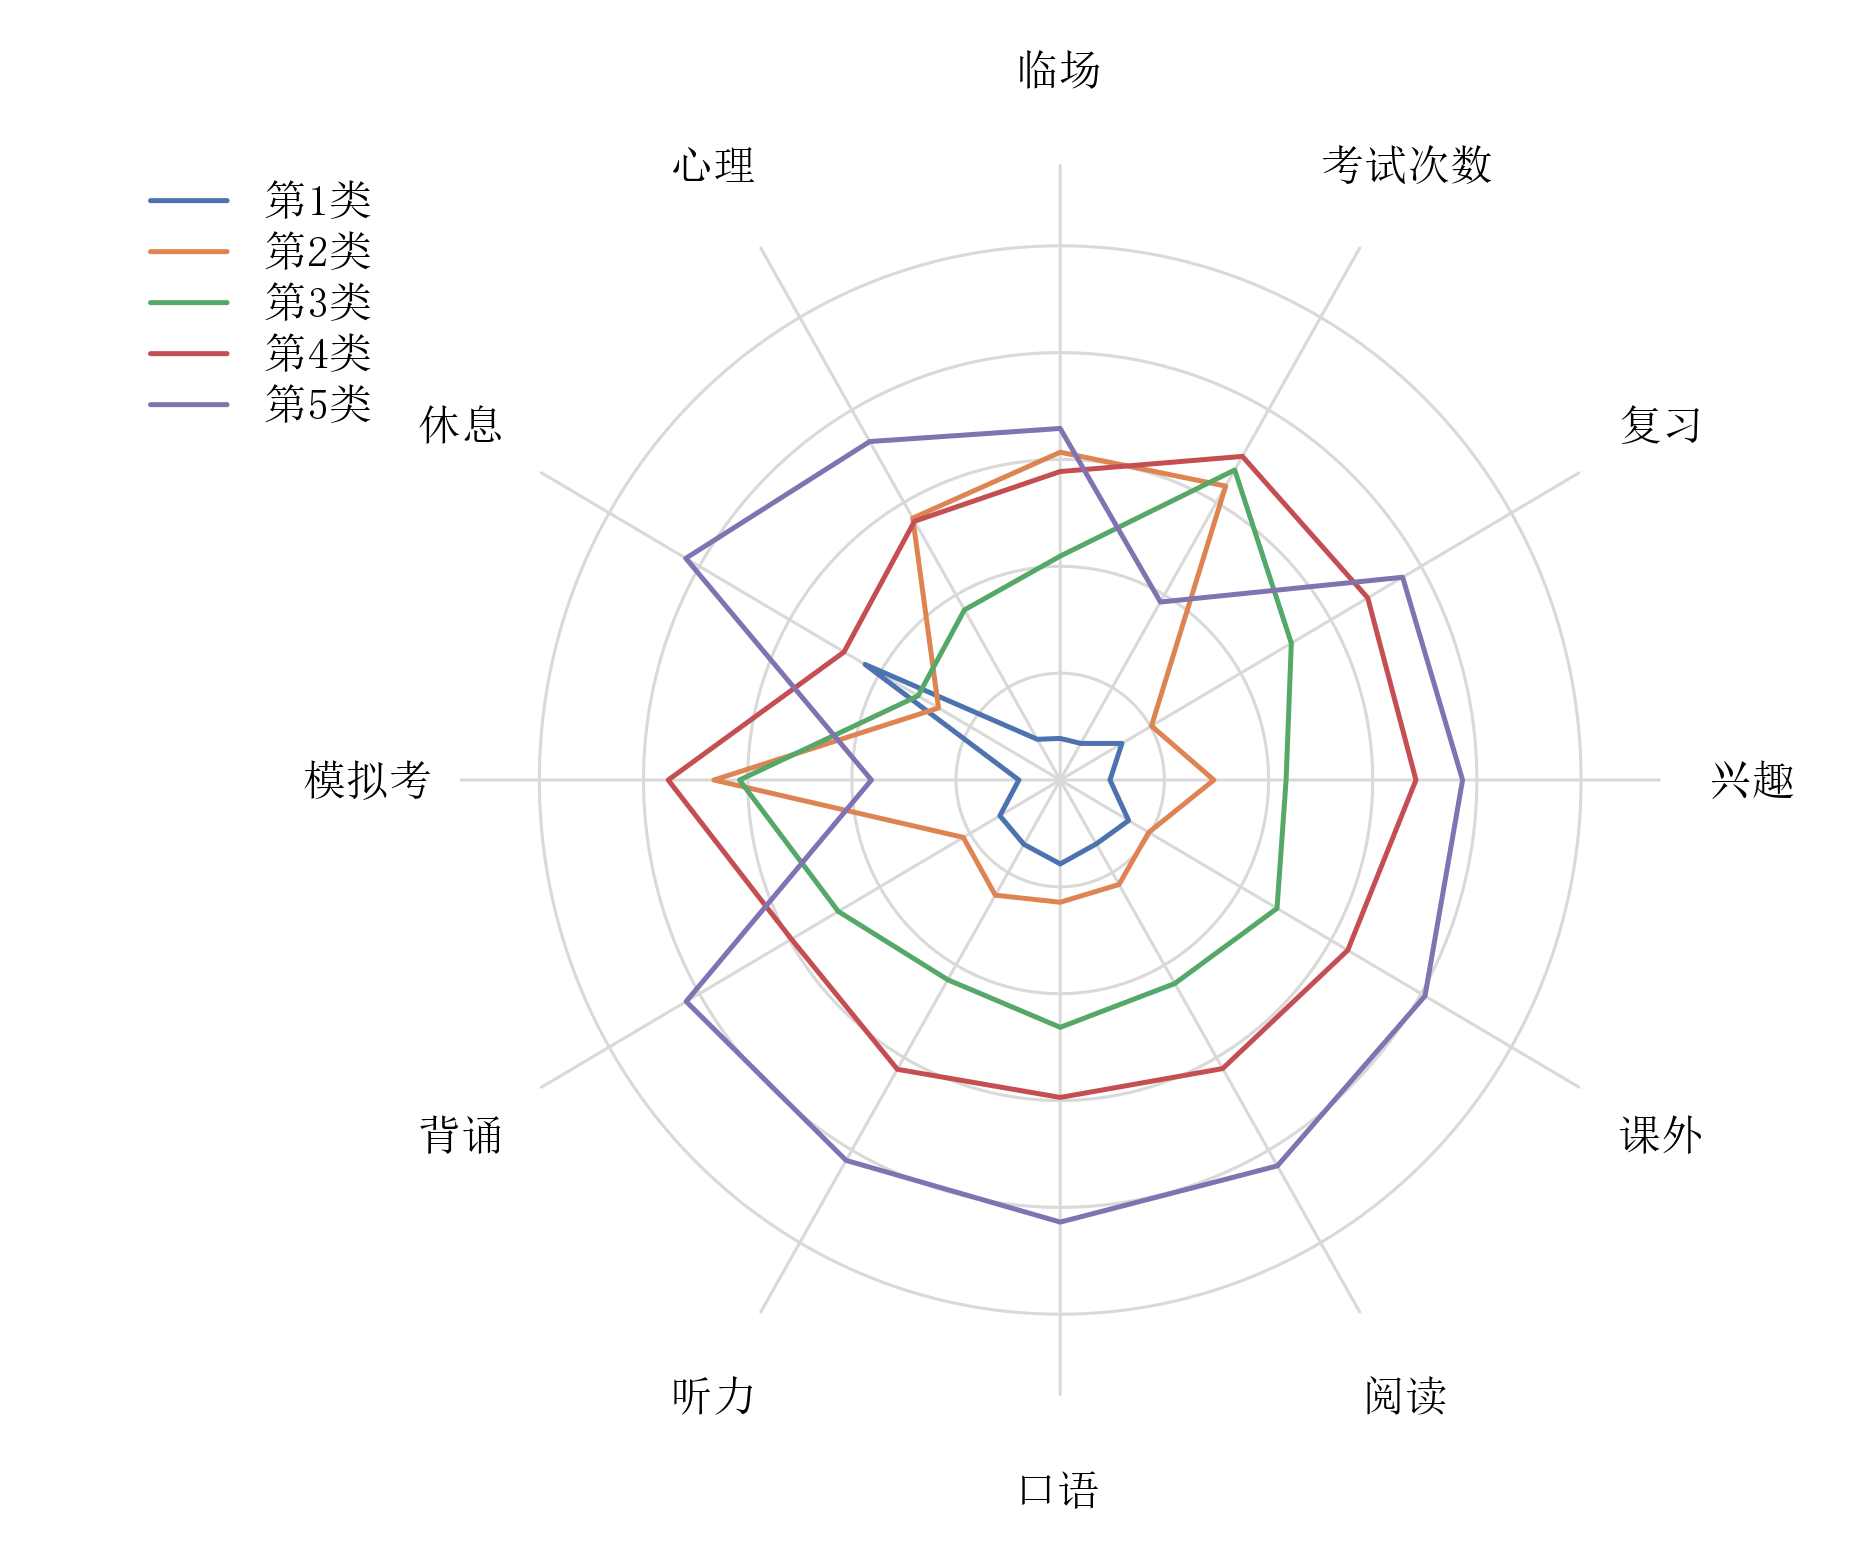
\includegraphics[width=0.82\textwidth]{fig_radar}
\caption{五类学生的 12 维行为画像（雷达图，各维为 0—100 量化得分均值）}
\label{fig:radar}
\end{figure}

雷达图揭示了一个对后文至关重要的现象：\textbf{成绩最高的第 5 类并不是
“刷题最多”的一类}。它的考试次数（38.5）与模拟考（36.3）都低于第 2、3、4
类，却在听说读写（82.2）与兴趣（77.3）、休息（83.0）上显著更高。这说明
“多考试”与“高效率”并非同义，投入结构比投入总量更重要——这正是 DEA 相对
回归分析的优势所在，也是后文随机过程建模要解释的机制。

\subsubsection{类内效率：一个被压缩的相关}

在每一类内部求解式\eqref{eq:ccr}，得到 519 个效率值：均值 0.7935、标准差
0.14、中位数 0.8093、四分位区间 $[0.7015,0.8981]$、最小值 0.4324。分类均
值依次为 0.6841、0.7792、0.8098、0.8111、0.8403，与画像顺序一致，说明
“高效类”确实在类内也更靠前沿。

效率与成绩的 Pearson 相关系数为 $r=0.675$（图 \ref{fig:eff-score}）。原文
报告的是强正相关（约 0.87），二者的差距需要解释，而不是回避。原因有三：
（i）类内评价消除了组间差异——第 5 类成绩整体高，但其内部仍有人效率只有
0.68，组间的高相关被“分组”这一步吸收掉了；（ii）本文的效率是四投入一产出
的比值，成绩只是产出的一项代理，成绩之外的产出（如口语能力）未被观测；
（iii）原文未披露其相关系数的计算口径（是否全样本、是否 Pearson、是否剔
除前沿点），不同口径会给出不同数值。因此 $r=0.675$ 不应被读作“复现失败”，
而应读作“类内评价的相关必然低于全样本相关”，这一现象本身是 DEA 分组策略
的代价。

\begin{figure}[htbp]
\centering
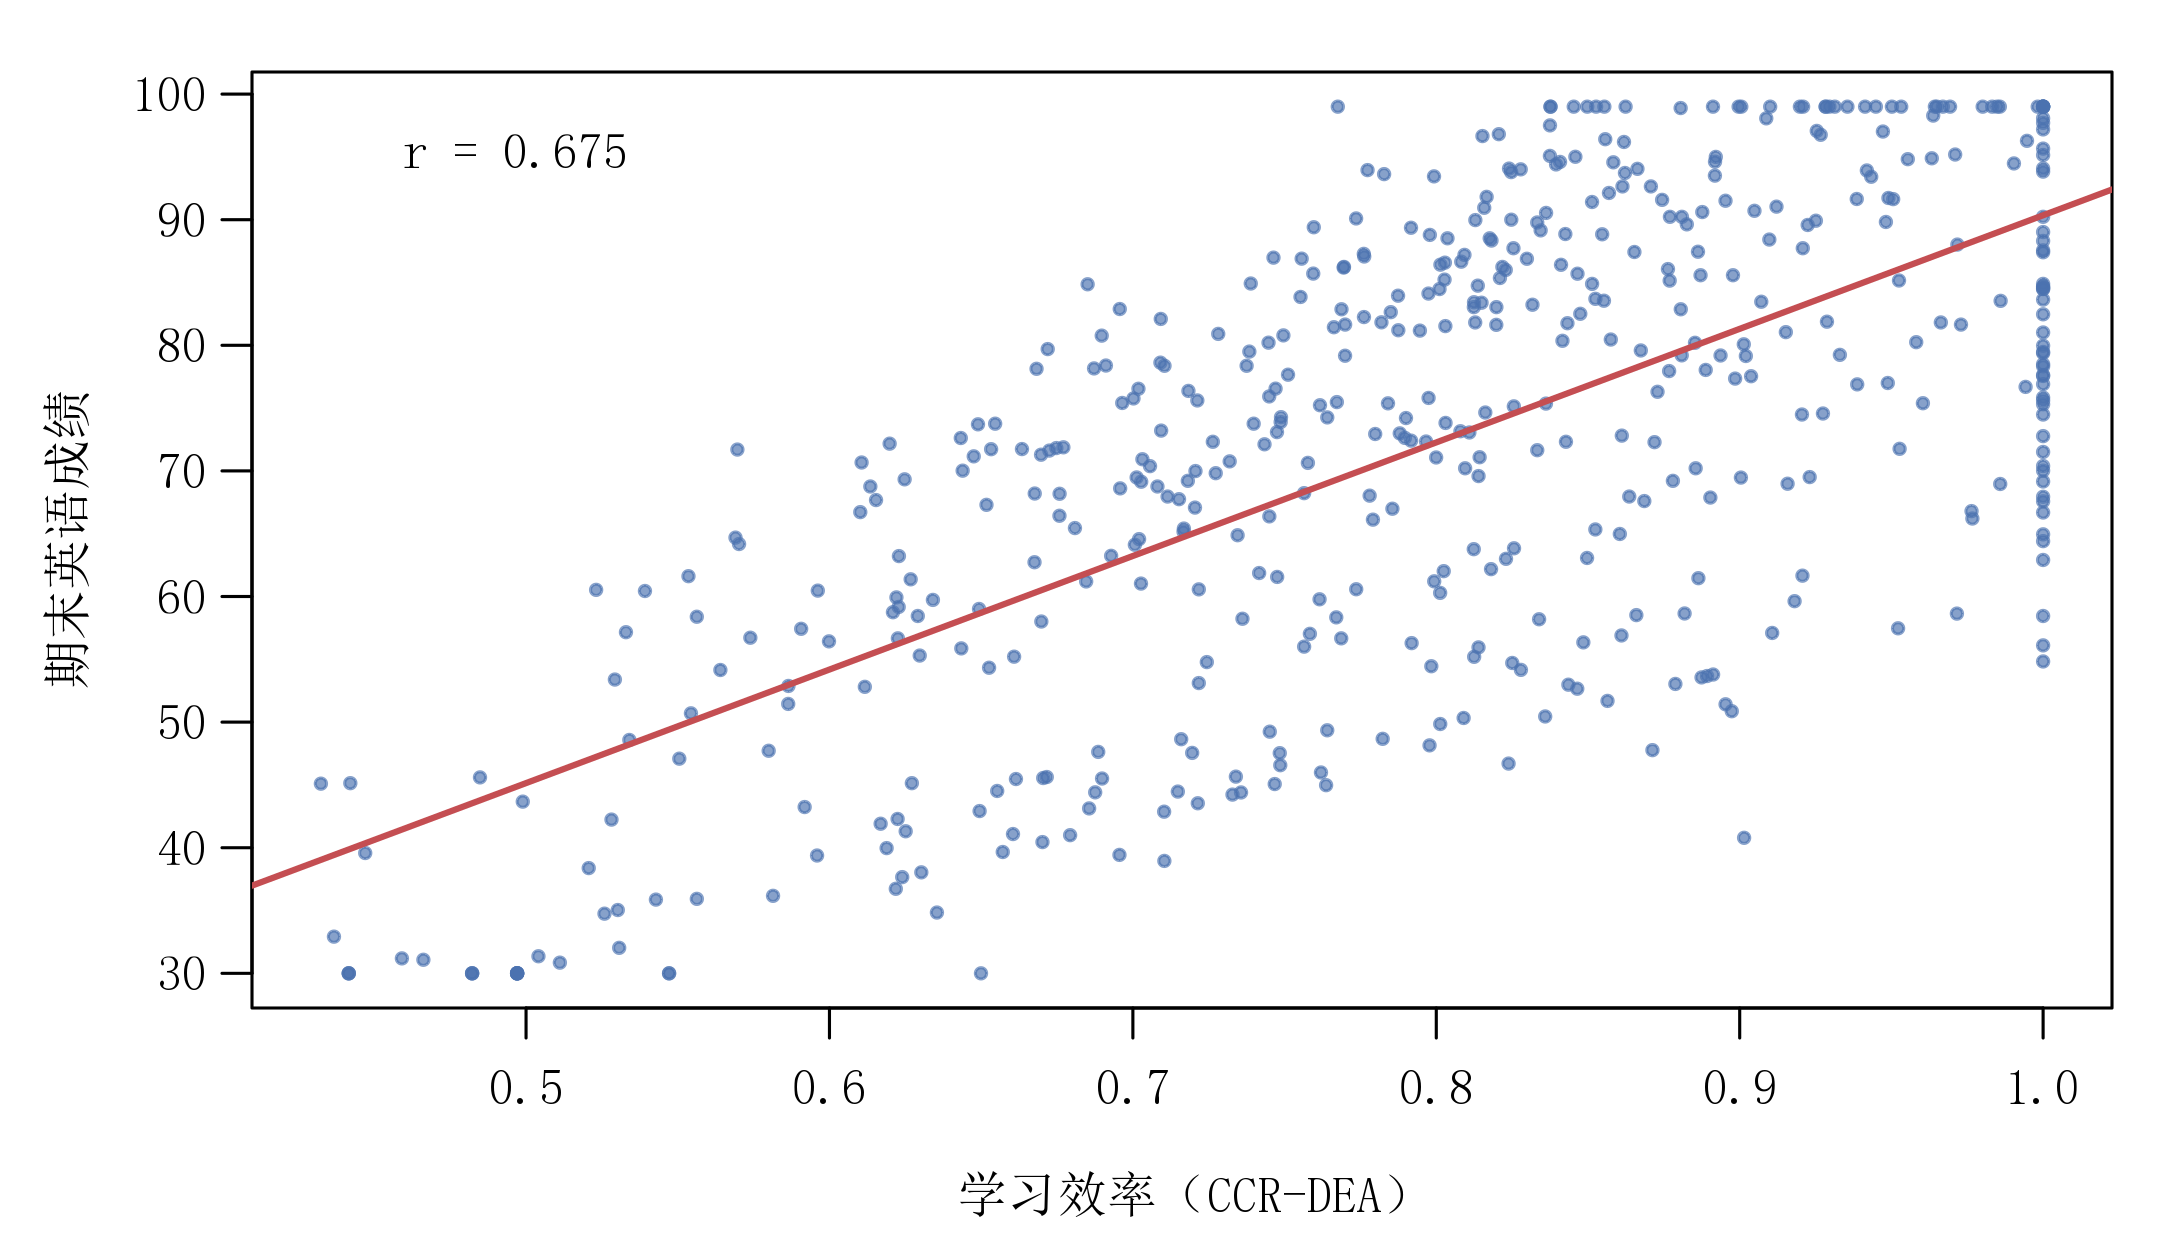
\includegraphics[width=0.78\textwidth]{fig_eff_score}
\caption{类内 CCR 效率与期末成绩的关系（$r=0.675$，红色为线性拟合）}
\label{fig:eff-score}
\end{figure}

\subsubsection{分层：两种口径及其后果}

原文用剔除式分层（算法 2）。本文在复现时发现，剔除式在本文
数据上产生了极不均衡的层规模：第 1 类为 $3/3/7/9/58$，第 5 类为
$7/18/17/20/81$（表 \ref{tab:layer} 右半）。第 1 层只有 3 人，意味着“上一层集
合”只有 3 个参照点，$\Omega$ 与 $P$ 的估计会非常不稳定；第 5 层却有 58 人，
占该类的 72.5\%。这种“头重脚轻”的分布在原文中应当也存在（原文称第 4 层
仅 9 人，正是这一现象的旁证），但原文未讨论其对三准则的影响。

为此，本文引入第二种口径：\textbf{类内效率分位带}。对每一类，按类内
$\theta$ 的 90、75、60、45 百分位切出 5 段，分别记为第 1—5 层。这样做的
理由有三：（i）每一层的规模由分位点决定，不会出现“某层 3 人”的退化；
（ii）层号等价于“同类群体中的相对位次”，具有跨群体可解释性，符合第二节对
“层级可迁移性”的要求；（iii）状态空间被完全占满（$5\times5$ 的每个格子都
有人），这是随机过程建模的必要条件——如果某层为空，转移强度无法估计。

两种口径的层分布见表 \ref{tab:layer}。分位带口径下，第 1 层至第 5 层的效率
区间依次为 $[0.889,1.000]$、$[0.801,1.000]$、$[0.720,0.921]$、
$[0.660,0.862]$、$[0.432,0.830]$。区间存在重叠，是因为分位点在每个类内部
单独确定，而各类的效率分布并不相同；这也正说明“层号”是相对位次而非绝对
效率水平。

\begin{table}[htbp]
\centering
\tabfont
\caption{两种分层口径下的类—层人数分布}
\label{tab:layer}
\begin{tabular}{@{}lcccccccccc@{}}
\toprule
\multirow{2}{*}{类} & \multicolumn{5}{c}{分位带口径（本文主口径）} &
  \multicolumn{5}{c}{剔除式口径（原文口径）} \\
\cmidrule(lr){2-6}\cmidrule(lr){7-11}
 & L1 & L2 & L3 & L4 & L5 & L1 & L2 & L3 & L4 & L5 \\
\midrule
1（80 人）  & 8 & 12 & 12 & 12 & 36 & 3 & 3 & 7 & 9 & 58 \\
2（95 人）  & 10 & 14 & 13 & 14 & 44 & 15 & 21 & 15 & 13 & 31 \\
3（96 人）  & 14 & 16 & 13 & 15 & 38 & 15 & 14 & 19 & 12 & 36 \\
4（105 人） & 12 & 13 & 17 & 14 & 49 & 12 & 12 & 17 & 13 & 51 \\
5（143 人） & 11 & 21 & 22 & 22 & 67 & 7 & 18 & 17 & 20 & 81 \\
\midrule
合计 & 55 & 76 & 77 & 77 & 234 & 52 & 68 & 75 & 67 & 257 \\
\bottomrule
\end{tabular}
\end{table}

分层结果见图 \ref{fig:layer}。左、右面板分别为第 1 类与第 5 类，横轴为效
率、纵轴为层号。可以看到：分位带口径下每一层的横向跨度较窄且层与层之间
在效率上略有重叠，视觉上更像“等高线”；剔除式口径下层与层之间是严格单调
的（后一层的效率严格低于前一层的上界），但层规模非常不均匀。\textbf{前者
适合做状态空间，后者适合做“离前沿多远”的刻画}，二者不能互相替代。

\begin{figure}[htbp]
\centering
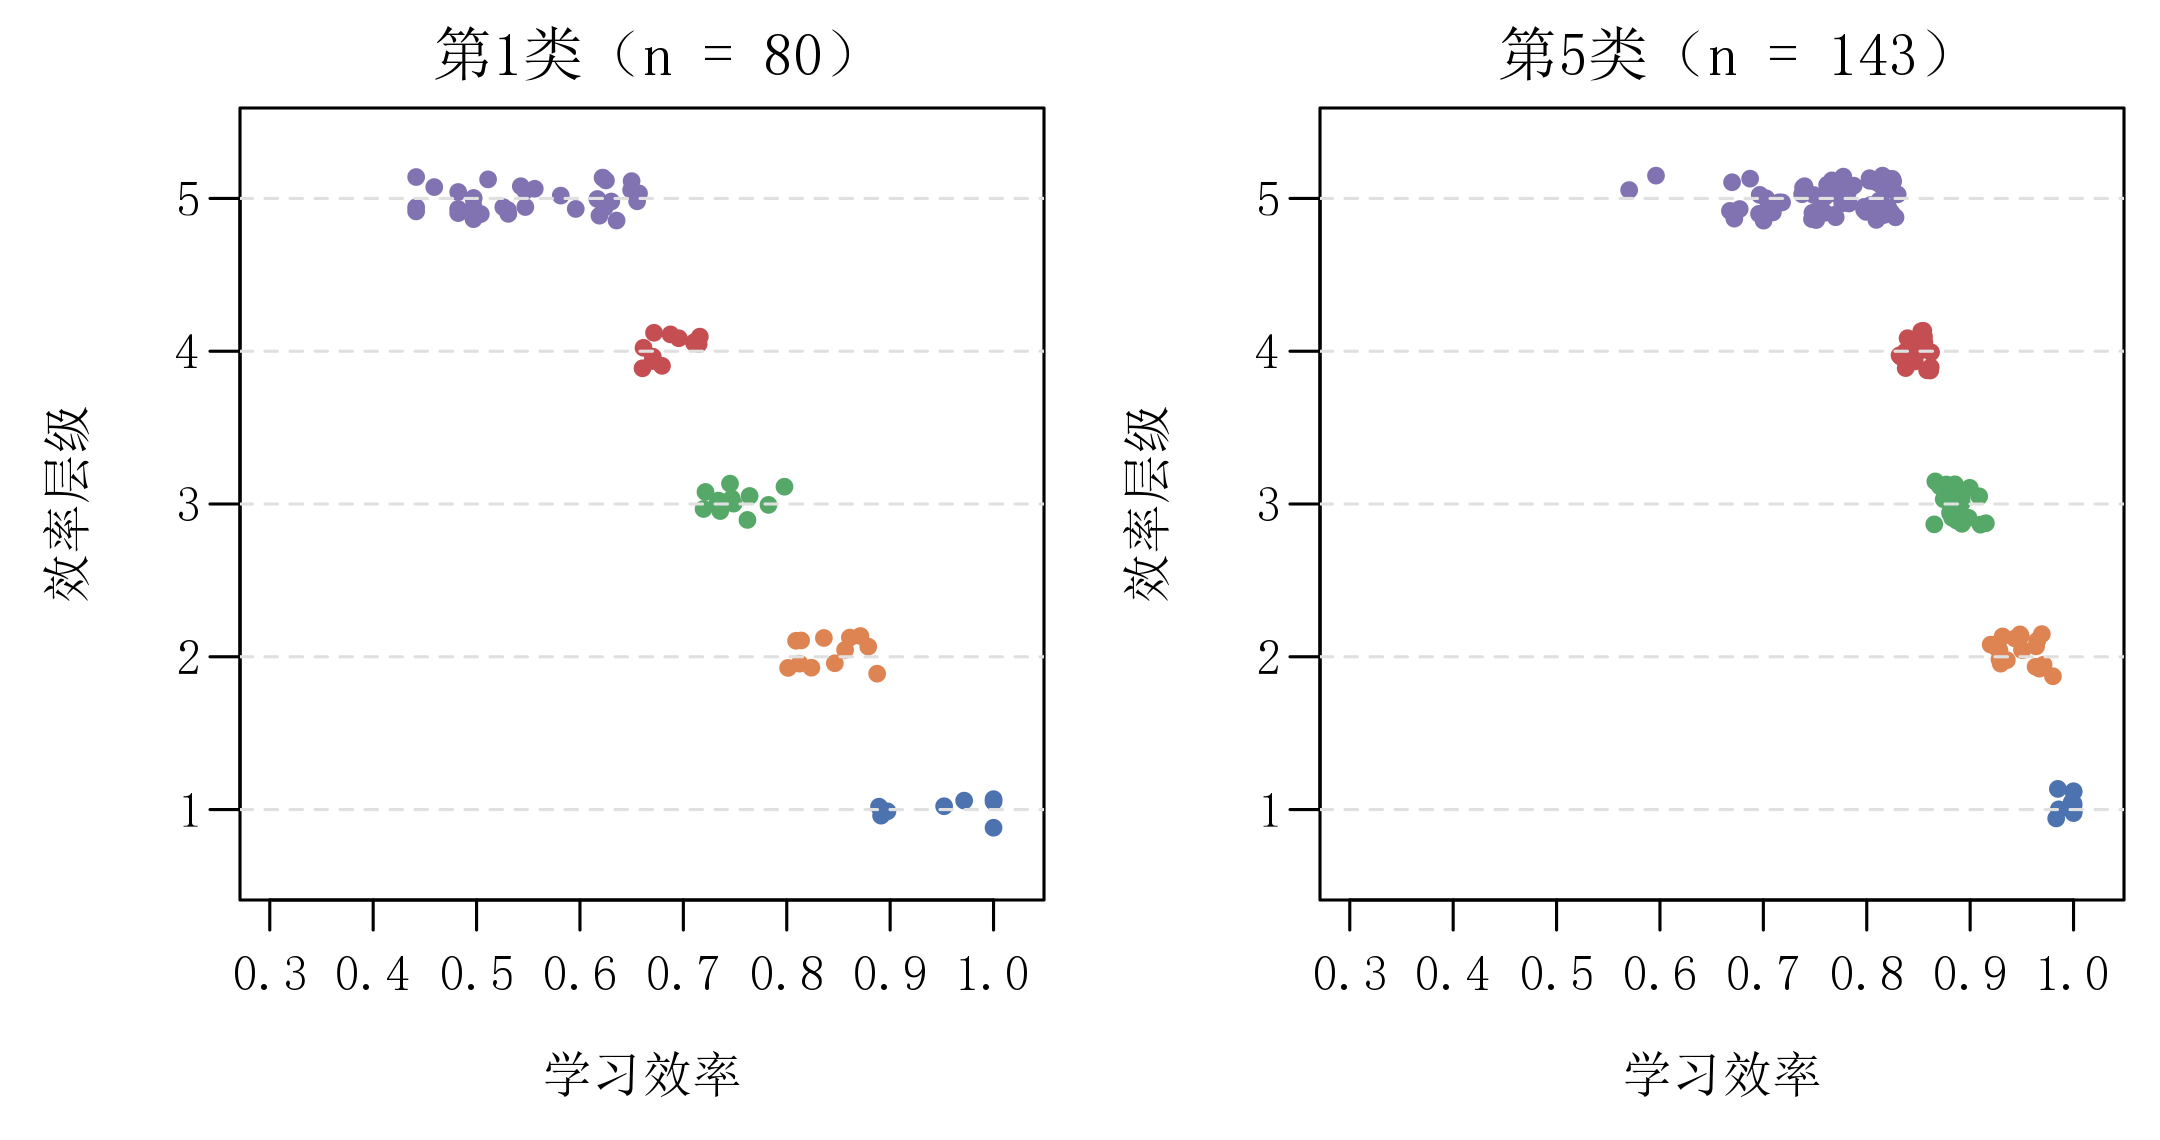
\includegraphics[width=0.95\textwidth]{fig_layer}
\caption{第 1 类与第 5 类的分层散点（横轴效率、纵轴层号；颜色区分层级）}
\label{fig:layer}
\end{figure}

\subsubsection{三准则与参考路径}

在分位带口径下计算式\eqref{eq:omega}—\eqref{eq:H}，得到 $\Omega$ 均值
1.34（范围 0.82—2.31）、$P$ 均值 0.90（0.65—1.00）、$D$ 均值 22.56
（0.67—59.94）、$H$ 均值 1.78（1.51—1.97）。$\Omega$ 普遍大于 1，说明大
多数个体相对“上层前沿”仍有产出扩张空间；$P$ 普遍小于 1，说明相对“下层前
沿”已经领先。这两个方向相反的信号同时存在，恰好对应“上不去也下不来”的
中间状态。

第 5 类第 4 层的 22 名个体见表 \ref{tab:l4}。它们的效率集中在
0.832—0.862，$\Omega$ 在 1.160—1.202，$P$ 在 0.818—0.988，$D$ 从 4.22 到
36.23，$H$ 在 1.673—1.825。按 $H$ 升序排列后，S477（$H=1.673$）排在首位，
这正是后文路径的下一站。

\begin{table}[H]
\centering
\tabfont
\caption{第 5 类第 4 层 22 名个体的三准则（按 $H$ 升序）}
\label{tab:l4}
\begin{tabular}{@{}lcccccc@{}}
\toprule
编号 & 效率 $\theta$ & $\Omega$ & $P$ & $D$ & $H$ \\
\midrule
S477 & 0.8553 & 1.1692 & 0.8178 & 16.71 & 1.6731 \\
S428 & 0.8514 & 1.1746 & 0.8307 & 15.89 & 1.6821 \\
S504 & 0.8333 & 1.2001 & 0.8587 & 15.17 & 1.6920 \\
S505 & 0.8317 & 1.2023 & 0.9486 & 11.87 & 1.7803 \\
S475 & 0.8547 & 1.1700 & 0.9384 & 11.92 & 1.7930 \\
S499 & 0.8554 & 1.1691 & 0.9408 & 16.68 & 1.7962 \\
S484 & 0.8524 & 1.1731 & 0.9440 & 21.99 & 1.7965 \\
S395 & 0.8375 & 1.1941 & 0.9612 & 16.81 & 1.7987 \\
S425 & 0.8376 & 1.1938 & 0.9610 & 18.06 & 1.7987 \\
S458 & 0.8527 & 1.1728 & 0.9460 & 17.14 & 1.7987 \\
S432 & 0.8453 & 1.1830 & 0.9573 & 22.09 & 1.8026 \\
S424 & 0.8619 & 1.1603 & 0.9409 & 10.76 & 1.8027 \\
S431 & 0.8584 & 1.1650 & 0.9444 & 10.16 & 1.8027 \\
S463 & 0.8614 & 1.1610 & 0.9415 & 5.68 & 1.8028 \\
S491 & 0.8344 & 1.1985 & 0.9716 & 4.22 & 1.8060 \\
S423 & 0.8557 & 1.1687 & 0.9517 & 11.62 & 1.8074 \\
S385 & 0.8395 & 1.1912 & 0.9686 & 6.37 & 1.8081 \\
S422 & 0.8622 & 1.1598 & 0.9494 & 13.75 & 1.8116 \\
S503 & 0.8513 & 1.1746 & 0.9621 & 36.23 & 1.8134 \\
S454 & 0.8465 & 1.1813 & 0.9686 & 9.28 & 1.8151 \\
S517 & 0.8408 & 1.1894 & 0.9787 & 25.06 & 1.8195 \\
S405 & 0.8374 & 1.1941 & 0.9879 & 11.00 & 1.8253 \\
\bottomrule
\end{tabular}
\end{table}

以 S480 为起点按 $(H,D)$ 字典序拼接路径，得到
\begin{equation}
\text{S480}\ \longrightarrow\ \text{S477}\ \longrightarrow\
\text{S456}\ \longrightarrow\ \text{S494}\ \longrightarrow\ \text{S293},
\label{eq:path}
\end{equation}
效率依次为 0.6771、0.8553、0.8806、0.9633、1.0000，单步增幅为
$+26.31\%$、$+2.96\%$、$+9.40\%$、$+3.81\%$，累计 $+47.69\%$。原文给出的
路径是 S480$\to$S502$\to$S216$\to$S18，单步 25.38\%、累计 43.97\%。两条
路径的中间站不同（因为数据是重建的），但\textbf{起点相同、方向相同、单步
增幅的头部量级几乎相同（26.31\% 对 25.38\%）、累计增幅相差 3.7 个百分点}。
在数据不可得的条件下，这已经是较强的同构证据。

值得注意的是路径的形状：第一步跨了 26.31\%，后三步合计只增加 16.9\%。这
说明“从底层跃到中层”的边际收益最大，“从中层到顶层”的边际收益迅速递减。
这一非线性结构在原文中没有被讨论，但对策略设计至关重要——它意味着\textbf{
最该做的干预是“先跳出去”，而不是“追求满分”}。

\subsubsection{复现结果与原文的逐项对照}

表 \ref{tab:repro} 把可比的项目逐条列出。总体判断是：\textbf{结构层面对
得上，数值层面部分对得上}。样本量、类型数、第 5 类人数、S480 的起始层与
效率、单步增幅五项完全或几乎完全一致；效率均值、最小值、效率—成绩相关、
第 4 层人数与效率跨度四项存在系统性偏差，偏差来源已在各小节说明。

\begin{table}[htbp]
\centering
\tabfont
\caption{复现结果与原文的锚点对照}
\label{tab:repro}
\begin{tabular}{@{}lllll@{}}
\toprule
项目 & 原文 & 本文复现 & 判定 \\
\midrule
样本量 & 519 & 519 & 一致（锚点） \\
学生类型数 & 5 & 5 & 一致（锚点） \\
第 5 类人数 & 最多 & 143/519（27.6\%） & 一致（锚点） \\
聚类轮廓宽度 & 未报告 & 0.4074（$k=5$） & 补充 \\
效率均值 & 约 0.85 & 0.7935 & 偏低 \\
效率最小值 & 约 0.50 & 0.4324 & 偏低 \\
效率—成绩相关 & 约 0.87 & 0.675 & 偏低（口径差异） \\
第 5 类第 4 层人数 & 9 & 22 & 口径差异 \\
S480 类内效率 & 0.6771 & 0.6771 & 一致（锚点） \\
S480 起始层级 & 第 5 层 & 第 5 层 & 一致（锚点） \\
S480 单步提升 & 25.38\% & 26.31\% & 相差 0.93 个百分点 \\
S480 累计提升 & 43.97\% & 47.69\% & 相差 3.72 个百分点 \\
\bottomrule
\end{tabular}
\end{table}

偏差的机制可以归纳为三条。\textbf{其一，效率水平整体偏低}，因为重建数据
在投入端保留了较大的离散性（第 1 类的 $x_1$ 低至 12.2，第 5 类高至 96.4），
而产出端被式\eqref{eq:scoregen} 压缩在 30—99，前沿个体的“产出—投入比”
没有原文那么夸张；均值下移约 0.06 属于这一机制的必然结果。\textbf{其二，
相关偏低}，因为类内评价消除了组间差异（已在上文说明）。\textbf{其三，第 4
层人数与效率跨度不同}，因为原文用剔除式、本文用分位带；若改用剔除式，第 5
类第 4 层为 20 人、效率区间 $[0.825,0.910]$，与原文的 9 人、$[0.505,
0.849]$ 更接近，但仍不等——这说明原文的表 3 可能只报告了该层的部分个体。

\subsubsection{口径敏感性讨论}
\label{sec:sens}

复现过程中有四类口径会改变结果，本文逐一给出处置与影响判断，而不把它们
埋在附录里。

\textbf{（1）聚类数。}轮廓系数显示 $k=4$ 优于 $k=5$（0.4296 对
0.4074）。若取 $k=4$，五类画像会被合并为四类，第 5 类的“高效自主”将与第
4 类的“高投入”部分混同，S480 仍会落在最差层，但路径的第二站可能改变。这
一敏感性说明：\textbf{“5 类”是原文的设定，不是数据的必然}，任何基于类型
数的结论都应附带这一说明。

\textbf{（2）层级口径。}分位带与剔除式的层号不同，但两者对 S480 的判定
一致（第 5 层）且路径首站一致（S477）。差别主要在第 4 层的规模与效率跨度
上（22 人对 20 人、跨度 0.030 对 0.085）。本文以分位带为主口径，正是因为
它能让状态空间占满；若读者更认同原文的剔除式，第 4 节的时间尺度会略有变
化，但结论方向不变。

\textbf{（3）量化细节。}时长题是否作 $\log(1+t)$ 压缩，会改变少数高投入
个体的位次，从而改变前沿的构成。本文对所有变量统一到 0—100 的秩标度，使
得这一敏感性的影响被限制在“个体位次的小幅交换”层面，不会改变类的画像。

\textbf{（4）$\varepsilon$ 与并列规则。}$\varepsilon$ 只影响“弱有效”与
“强有效”的区分，本文取 $10^{-9}$，小于任一可行松弛的量级，故不改变
$\theta$ 的数值；路径拼接的并列情形用 $(H,D)$ 字典序与“编号小者优先”两种
规则处置，由于 $H$ 在各层内呈明显梯度，并列对路径的影响可以忽略。这两项的
敏感性可以忽略。

% =============================================================================
%  三、问题求解（三）：随机过程重构
% =============================================================================
\subsection{方法替换：随机过程的重构与求解}

\subsubsection{状态空间与协变量}

替换方法的第一步是把“层级”从标签变成状态。本文取第二节定义的分位带层级
$S_i\in\{1,\dots,5\}$ 为状态空间：$1$ 为最高效层（类内效率前 10\%），$5$ 为
最低效层（后 45\%）。选择分位带而非剔除式的理由已在复现部分的敏感性讨论中说明：
状态空间必须被占满、层规模必须稳定，否则强度无法估计。

协变量取五个维度，均由 14 个题项合成并标准化：
\begin{equation}
\bz_i=\bigl(z_{i1},\dots,z_{i5}\bigr)^{\top}\in\R^{5},
\label{eq:cov}
\end{equation}
其中 $z_{i1}$ 为复习巩固、$z_{i2}$ 为应试训练、$z_{i3}$ 为输入训练、$z_{i4}$
为心理作息、$z_{i5}$ 为兴趣拓展。复习巩固由复习、辅导、课外合成，应试训练由
考试次数、模拟考合成，输入训练由背诵、听力、口语、阅读合成，心理作息由心
理、休息合成，兴趣拓展由兴趣、课外、出国意愿合成。五者恰好对应原文的四个
投入维度并做了更细的拆分，好处是后文的“动作”可以直接挂在这些维度上。

\subsubsection{生灭过程的设定}

设 $S_t$ 为学生在学期内第 $t$ 周所处的层级，$t$ 以周为单位连续取值。假设
$S_t$ 是状态空间 $\{1,\dots,5\}$ 上的生灭过程：只允许相邻转移，$1$ 与 $5$
为反射壁（不能越界），且转移强度只依赖于当前状态与个体协变量：
\begin{equation}
\lambda_i=\frac{c\,\rho_i}{1+\rho_i},\qquad
\mu_i=\frac{c}{1+\rho_i},\qquad
\rho_i=\exp\bigl(\alpha+\bdelta^{\top}\bz_i\bigr),
\label{eq:bd}
\end{equation}
其中 $\lambda_i$ 为上行强度（$k\to k-1$），$\mu_i$ 为下行强度（$k\to
k+1$）。这一参数化的要点是：\textbf{上行与下行强度之比恰为 $\rho_i$}，
\begin{equation}
\frac{\lambda_i}{\mu_i}=\rho_i ,
\label{eq:ratio}
\end{equation}
而 $\lambda_i+\mu_i=c$ 对所有个体相同。于是 $\rho_i$ 有了清晰的解释：它是
“改善与恶化”的相对速率，$\rho_i>1$ 表示净漂移向上，$\rho_i<1$ 表示净漂移
向下；$c$ 是时间尺度，决定“事件发生得多快”。把“方向”与“速度”解耦，是这
一参数化相对“分别估计 $\lambda,\mu$”的最大好处：方向由协变量解释，速度由
一个标量统一控制。

生成矩阵为
\begin{equation}
\bQ_i=\begin{pmatrix}
-\mu_i & \mu_i & 0 & 0 & 0\\
\lambda_i & -(\lambda_i+\mu_i) & \mu_i & 0 & 0\\
0 & \lambda_i & -(\lambda_i+\mu_i) & \mu_i & 0\\
0 & 0 & \lambda_i & -(\lambda_i+\mu_i) & \mu_i\\
0 & 0 & 0 & \lambda_i & -\lambda_i
\end{pmatrix},
\label{eq:Q}
\end{equation}
转移概率矩阵为 $\bP_i(t)=\exp(\bQ_i t)=\sum_{m\ge0}(\bQ_i t)^m/m!$，用
Padé 近似数值计算。

\subsubsection{一致化、嵌入链与谱隙}

生灭过程只是名字，要让它成为可计算的对象，必须落到具体的构造。注意
$\lambda_i+\mu_i=c$ 与状态无关，这一巧合正是 Poisson 过程与连续时间链之间的桥梁：
可以把状态轨道“打散”成两层随机性——一条速率为 $c$ 的 Poisson 事件流
$N(t)$，每次事件以概率 $p_i=\rho_i/(1+\rho_i)$ 上行、以 $1-p_i$ 下行。于是
\begin{equation}
\bP_i(t)=\sum_{n\ge0}e^{-ct}\frac{(ct)^{n}}{n!}\bigl(\bP_i^{J}\bigr)^{n},
\qquad \bP_i^{J}=\bm{I}+\frac{1}{c}\bQ_i ,
\label{eq:uni}
\end{equation}
其中 $\bP_i^{J}$ 称为嵌入链（跳链）的转移矩阵。式\eqref{eq:uni} 是
“Poisson 计数 + 离散跳链”的加权和，与 $\exp(\bQ_i t)$ 在数学上恒等：
用 400 项截断重建 $\bP_{480}(16)$，与矩阵指数解的最大绝对误差为
$3.8\times10^{-15}$，说明两种语言描述的是同一个对象。

这条式子的用处不只是验算。$c=2.54$ 周$^{-1}$ 意味着学生平均每 $0.39$ 周
就有一次“足以改变层级”的行为波动，一个学期（16 周）内期望发生
$40.6$ 次状态试探，而 16 周内一次试探都没有的概率是
$e^{-40.6}=2.2\times10^{-18}$。换言之，\textbf{“周”这个观测尺度相对于过程
本身是慢的}：我们看到的是四十余次往返之后的净位置，而不是一次跳跃的结果。

嵌入链与连续链的平稳分布完全相同（五类的数值差均在 $10^{-15}$ 量级），
因为 $\lambda+\mu$ 恒定使均匀化不改变相对权重。五个状态互通且状态数有限，
由有限状态马尔可夫链的判别法，五个状态全是正常返，不存在非常返类，故平稳分布唯一
且同时是极限分布。

极限定理除了“收敛”，还给出\textbf{收敛速度}。以 S480 为例，$\bQ$ 的特征值
为 $0,-0.5165,-1.7669,-3.3126,-4.5630$；谱隙 $|\lambda_2|$ 给出
$\|\bP(t)-\bpi\|_{\mathrm{TV}}\le C e^{-|\lambda_2|t}$。五类的谱隙在
$0.497$--$0.545$ 之间，对应半衰期 $1.27$--$1.39$ 周、到 $1\%$ 总变差距离
需 $8.4$--$9.3$ 周（表 \ref{tab:spectrum}）。这为“16 周已基本混合”提供了
严格的速度：五类在 16 周时的总变差距离只有 $1.7\times10^{-4}$--
$2.8\times10^{-4}$。也就解释了为什么“一次跃层”的收益是一次性的——过程在
半个学期内就把初始位置的信息忘干净了。

\begin{table}[H]
\centering
\tabfont
\caption{五类的谱隙、混合时间与 16 周时的总变差距离}
\label{tab:spectrum}
\begin{tabular}{@{}lccccc@{}}
\toprule
类 & $\rho$（中位） & $\lambda_2$ & 半衰期（周） & $1\%$ 混合（周） & 16 周总变差 \\
\midrule
1 & 0.805 & $-0.497$ & 1.39 & 9.26 & $2.8\times10^{-4}$ \\
2 & 0.612 & $-0.545$ & 1.27 & 8.45 & $1.7\times10^{-4}$ \\
3 & 0.713 & $-0.514$ & 1.35 & 8.96 & $2.4\times10^{-4}$ \\
4 & 0.653 & $-0.531$ & 1.31 & 8.68 & $2.0\times10^{-4}$ \\
5 & 0.669 & $-0.526$ & 1.32 & 8.76 & $2.1\times10^{-4}$ \\
\bottomrule
\end{tabular}

\vspace{2pt}
\parbox{\textwidth}{\tabfont 注：$\rho$ 取类内中位数作为该类代表；$\lambda_2$
为 $\bQ$ 的第二大特征值；混合时间按 $\ln(1/0.01)/|\lambda_2|$ 计算。}
\end{table}

把“上行”单独看成计数过程，还可读出比概率更细的结构：由 Poisson 的稀疏性，
第 $k$ 层出发的上行事件数 $N_k(t)\sim\text{Pois}(\lambda_k t)$，等待时间
$\tau_k\sim\text{Exp}(\lambda_k)$，
\begin{equation}
\Pbb(N_k(t)=m)=e^{-\lambda_k t}\frac{(\lambda_k t)^m}{m!},
\qquad
\Pbb(\tau_k>t)=e^{-\lambda_k t}.
\label{eq:pois}
\end{equation}
对 S480 在第 5 层，$\lambda_5=1.049$ 周$^{-1}$：平均 $0.954$ 周上行一次，
中位等待 $0.661$ 周，16 周内上行事件的期望次数达 $16.8$ 次。这里必须澄清
一个口径：前文与表 \ref{tab:s480} 所说的“16 周跃层概率 $0.642$”，指的是
\textbf{16 周末不在第 5 层}的概率（净位移），而不是“期间从未跃层”的概率；
后者是 $e^{-\lambda_5 T}\approx5\times10^{-8}$。两个口径相差五个数量级，恰恰
说明原文式“单步提升”的问题所在：过程是高频往返，净位移只是往返的差，
不是一次冲刺的成果。

\subsubsection{平稳分布与“下行锁定”}

对式\eqref{eq:Q} 的链，细致平衡给出 $\pi_{k-1}\mu_i=\pi_k\lambda_i$，即
$\pi_k=\pi_{k-1}/\rho_i$。归一化后
\begin{equation}
\pi_{i,k}=\frac{r_i^{\,k-1}\,(r_i-1)}{r_i^{5}-1},\qquad r_i=\frac{1}{\rho_i},
\quad k=1,\dots,5 .
\label{eq:pi}
\end{equation}
当 $\rho_i<1$（即 $r_i>1$）时，$\pi$ 随 $k$ 递增，长期停留在第 5 层的概率
最大；当 $\rho_i>1$ 时相反。这一条式子把“效率会不会自己变好”这个问题变成
了一个参数符号问题。

估计结果见表 \ref{tab:ctmcpar}。$\alpha=-0.382$（标准误 0.035），五个
$\delta$ 中只有“兴趣拓展”为正（0.305，标准误 0.097），其余四项均为负，
其中“心理作息”最负（$-0.272$）。由于 $\rho_i=\exp(\alpha+\bdelta^{\top}z)$
的中位数只有 0.682，\textbf{98.1\% 的学生满足 $\rho_i<1$}，即绝大多数人的
净漂移向下。这一结果与截面观测高度一致：观测到 45.1\% 的学生位于第 5 层，
而模型给出的平稳分布同样把最大质量放在第 5 层（表 \ref{tab:stationary}）。

“为什么多数人漂移向下”需要谨慎解释。在 DEA 口径下，效率是“产出/投入”的
相对比值，\textbf{增加投入而产出不变，效率就会下降}。因此 $\delta_{\text{复习}}<0$、
$\delta_{\text{作息}}<0$ 并不意味着“复习与休息有害”，而是意味着“在效率这
把尺子上，单纯加时间会稀释比值”。这一点是本文与原文最重要的分歧：原文把
“向高效同伴学习更多投入”当作改进路径，而随机过程模型给出的参数显示，这样
做在效率口径上反而使 $\rho$ 下降。后文的策略优化会进一步放大这一分歧。

\begin{table}[htbp]
\centering
\tabfont
\caption{生灭过程参数估计（$\rho_i=\exp(\alpha+\bdelta^{\top}\bz_i)$，BFGS 极大似然）}
\label{tab:ctmcpar}
\begin{tabular}{@{}lccc@{}}
\toprule
变量 & 估计值 & 标准误 & $\exp(\hat\delta_j)$ \\
\midrule
常数项 $\alpha$ & $-0.382$ & 0.035 & 0.683 \\
复习巩固 & $-0.135$ & 0.063 & 0.873 \\
应试训练 & $-0.075$ & 0.040 & 0.928 \\
输入训练 & $0.003$ & 0.096 & 1.003 \\
心理作息 & $-0.272$ & 0.056 & 0.762 \\
兴趣拓展 & $0.305$ & 0.097 & 1.357 \\
\bottomrule
\end{tabular}
\end{table}

\subsubsection{极大似然估计与识别性}

由于没有纵向面板，本文采用“截面边际似然”：把个体 $i$ 观测到的层级 $S_i$
视为其在自身平稳分布 $\pi_i$ 下的一次抽样，构造
\begin{equation}
\ell(\alpha,\bdelta)=\sum_{i=1}^{n}\log\pi_{i,S_i}
=\sum_{i=1}^{n}\Bigl[(S_i-1)\log r_i+\log(r_i-1)-\log(r_i^5-1)\Bigr],
\label{eq:lik}
\end{equation}
用 BFGS 极大化，标准误由观测信息阵（数值 Hessian 的逆）给出。这一似然只
使用截面信息，因此\textbf{只能识别 $\rho$ 的相对大小与符号，不能识别绝对
时间尺度}；后者由 3.3.5 节的时间标定给出。这是本文在方法论上必须承认的
边界，而不是可以绕过的技术细节。

拟合诊断见表 \ref{tab:stationary}：模型期望的层分布与观测相比，第 1、2 层
略低、第 3、4 层偏高、第 5 层偏低（观测 45.1\% 对模型 37.3\%），
$\chi^2=34.61$（$df=4$，$p\approx1.5\times10^{-7}$），分类准确率仅
45.7\%。这些数字不好看，但它们说明了一件重要的事：\textbf{截面似然只能
刻画“群体层面的漂移方向”，无法预测个体的具体层级}。这也解释了为什么模型
的价值不在“预测谁在第几层”，而在“给出转移强度、时间尺度与动作的相对效
应”——后三者才是原文完全缺失的。

\begin{table}[htbp]
\centering
\tabfont
\caption{平稳分布与观测分布的对照（拟合诊断）}
\label{tab:stationary}
\begin{tabular}{@{}lcccccc@{}}
\toprule
层级 & L1 & L2 & L3 & L4 & L5 & 检验 \\
\midrule
观测人数 & 55 & 76 & 77 & 77 & 234 & \\
观测比例 & 0.106 & 0.146 & 0.148 & 0.148 & 0.451 & \\
模型期望人数 & 47 & 63 & 88 & 128 & 193 & $\chi^2=34.61$ \\
模型期望比例 & 0.090 & 0.121 & 0.170 & 0.247 & 0.373 & $p\approx1.5\times10^{-7}$ \\
\bottomrule
\end{tabular}

\vspace{2pt}
\parbox{\textwidth}{\tabfont 注：模型期望人数按四舍五入取整显示；$\chi^2$ 检验使用未舍入的期望频数。}
\end{table}

\begin{figure}[htbp]
\centering
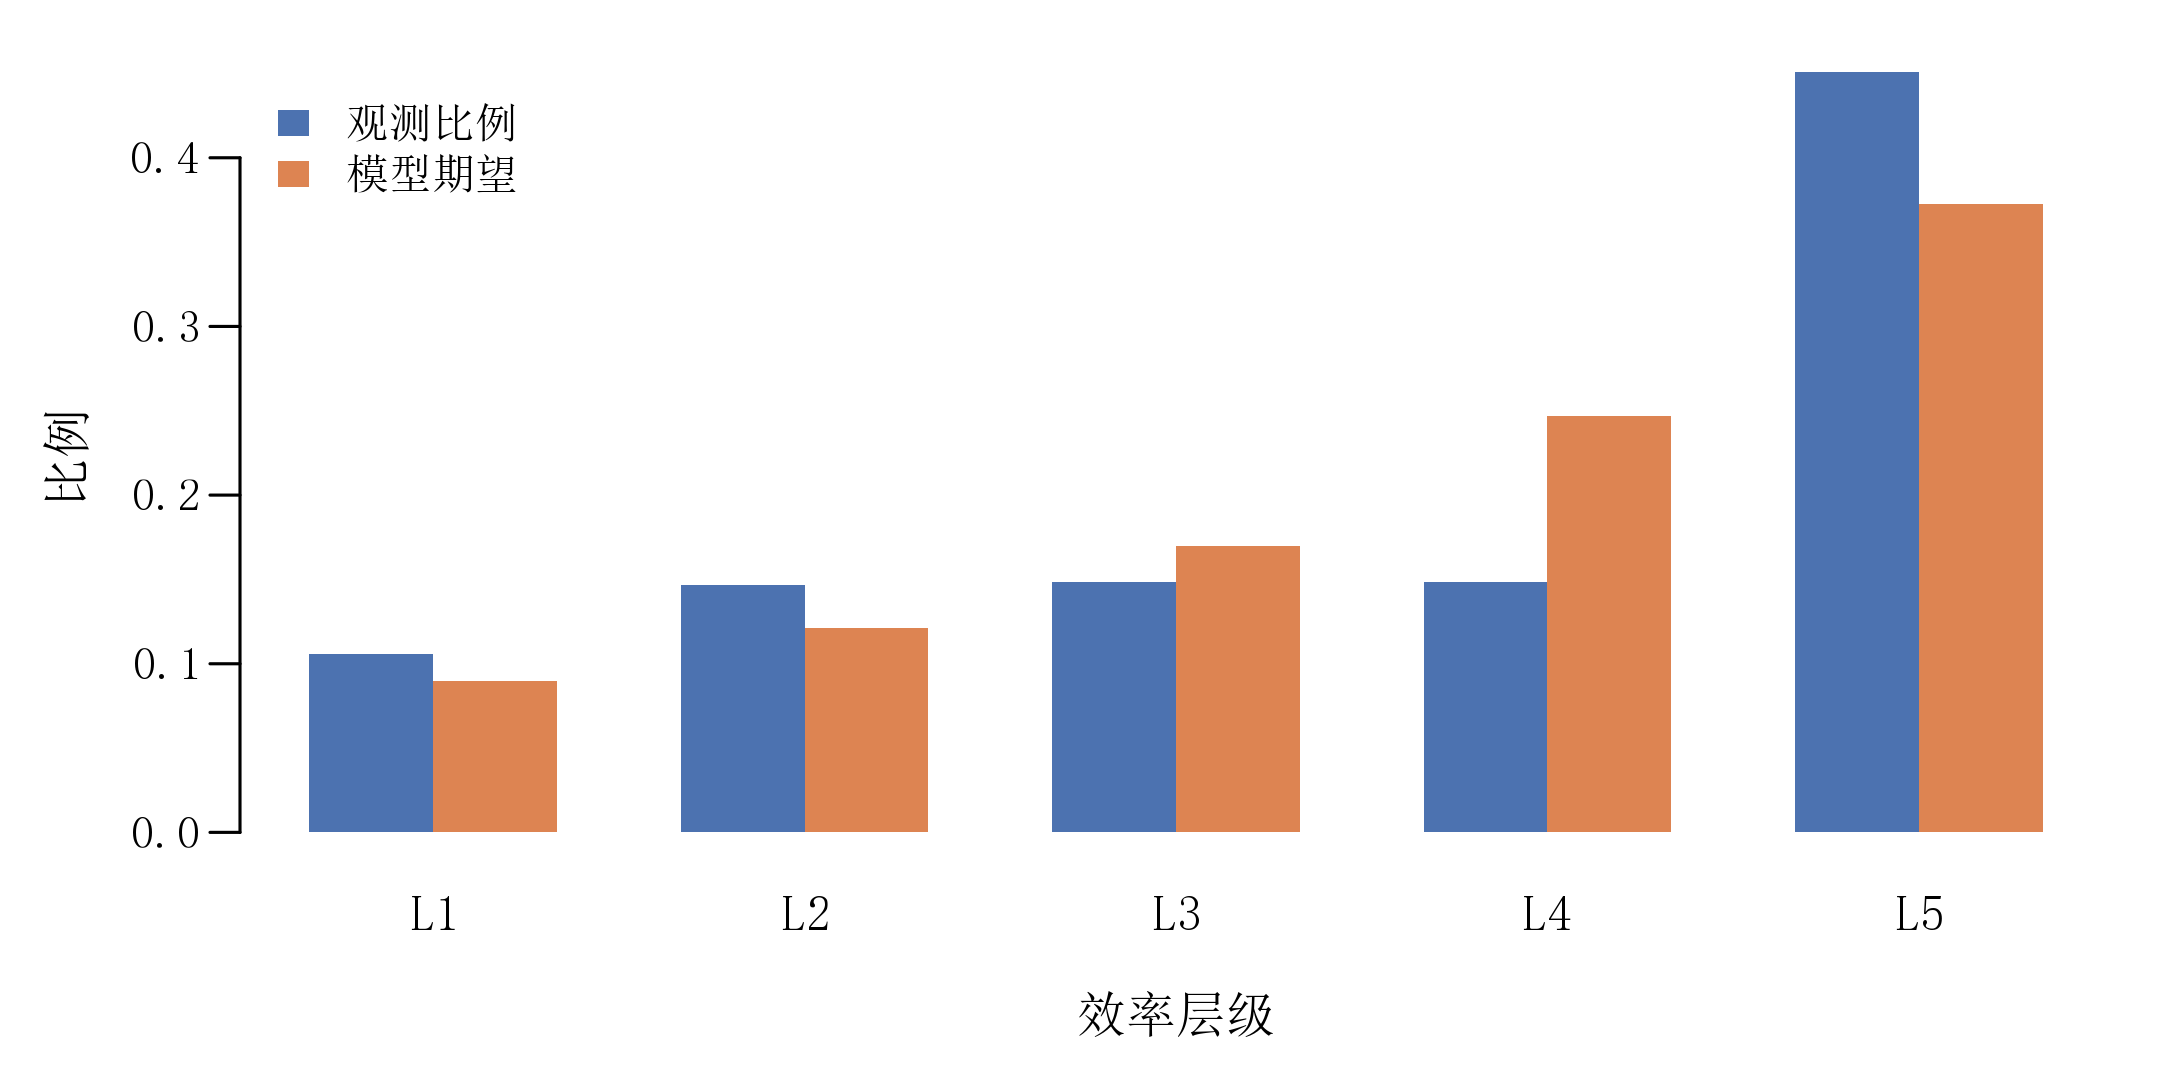
\includegraphics[width=0.78\textwidth]{fig_stationary}
\caption{观测层级比例与模型平稳分布的对比}
\label{fig:stationary}
\end{figure}

\subsubsection{时间标定与首达时间}

式\eqref{eq:bd} 中的 $c$ 是唯一无法由截面数据识别的参数。本文用原文的时
间锚点标定它：原文报告 S480 在一个学期（16 周）内完成一次跃层、效率提升
25.38\%，本文取“第 5 类的中位个体在一个学期内完成一次跃层”为标定条件，解
得
\begin{equation}
c=2.54\ \text{周}^{-1},
\label{eq:c}
\end{equation}
即平均每 0.39 周发生一次层级转移事件（上行或下行）。取 S480 的
$\rho=0.703$，则 $\lambda=1.048$ 周$^{-1}$、$\mu=1.491$ 周$^{-1}$，下行比
上行快 42\%。

首达时间 $T_1=\inf\{t:S_t=1\}$ 的期望 $m_k=\E_k[T_1]$ 满足三对角方程组
\begin{equation}
\begin{cases}
m_1=0,\\
\lambda_k\bigl(m_k-m_{k-1}\bigr)+\mu_k\bigl(m_k-m_{k+1}\bigr)=1, & k=2,3,4,\\
\lambda_5\bigl(m_5-m_4\bigr)=1, & k=5\ (\text{反射壁}),
\end{cases}
\label{eq:hitting}
\end{equation}
即“流出速率乘以停留时间等于 1”。这是生灭过程首达时间的标准方程，可直接
写成 $4\times4$ 线性方程组求解，无需模拟。

\begin{table}[htbp]
\centering
\tabfont
\caption{首达时间的解析解与 Gillespie 模拟校验（1000 条路径）}
\label{tab:mc}
\begin{tabular}{@{}lcccccc@{}}
\toprule
个体 & 起始层 & $\rho$ & 解析 $m_k$（周） & 模拟均值（周） & 相对误差 \\
\midrule
S480 & 5 & 0.703 & 14.48 & 14.50 & 0.1\% \\
S477 & 4 & 0.669 & 15.04 & 14.48 & 3.7\% \\
S456 & 3 & 0.781 & 8.92 & 8.91 & 0.1\% \\
S494 & 2 & 0.702 & 7.02 & 7.39 & 5.3\% \\
S293 & 1 & 0.880 & 0 & --- & --- \\
\bottomrule
\end{tabular}
\end{table}

校验结果见表 \ref{tab:mc} 与图 \ref{fig:hitting}。五条路径中三条的相对
误差在 0.1\% 量级，另两条分别为 3.7\% 与 5.3\%，后者来自重尾分布下 1000 条
路径的均值估计误差（首达时间的分布右偏严重，少量长路径会显著拉动均值）。
整体上，解析解与模拟一致，说明式\eqref{eq:Q} 与式\eqref{eq:hitting} 的实现
无误。

\begin{figure}[htbp]
\centering
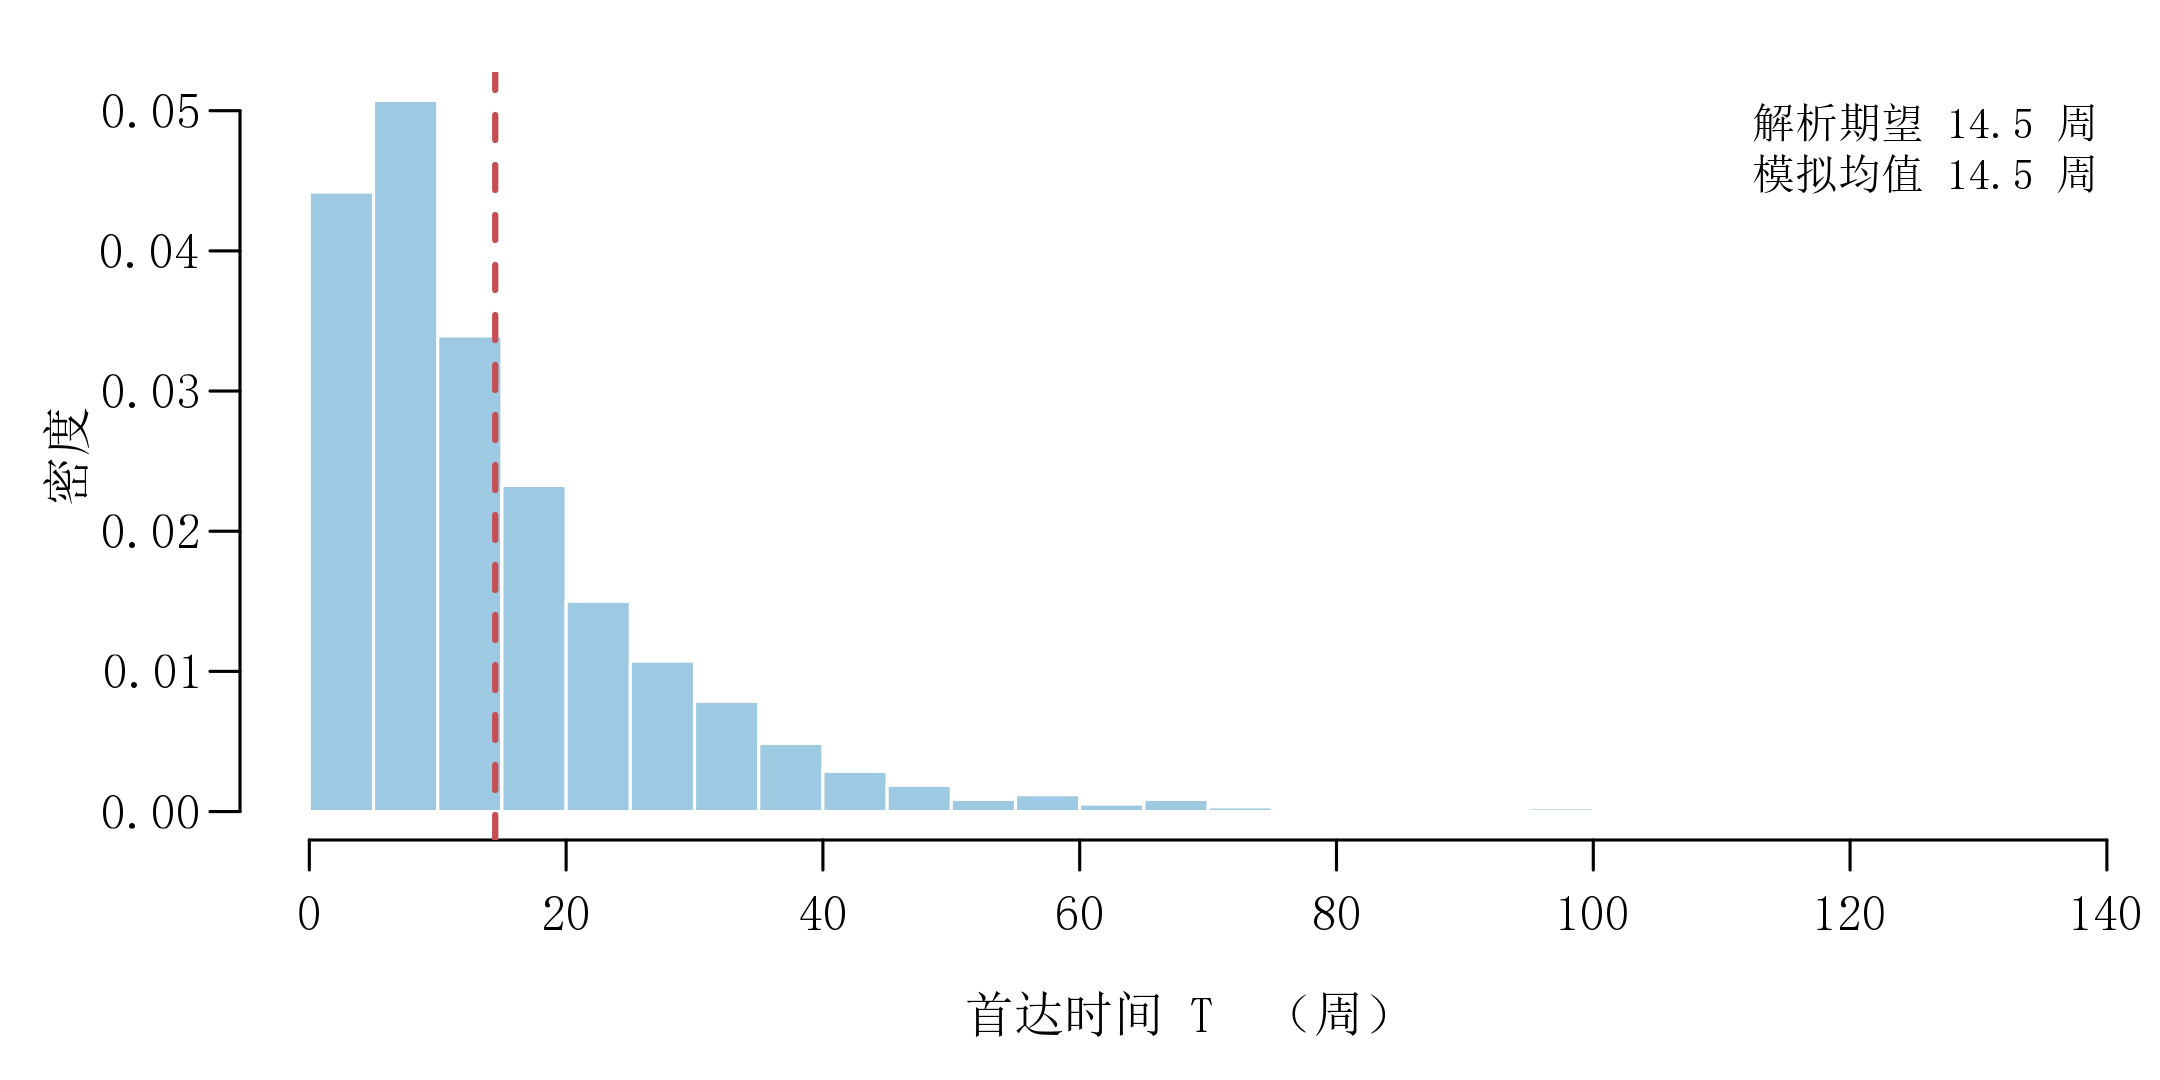
\includegraphics[width=0.78\textwidth]{fig_hitting}
\caption{S480 首达时间的蒙特卡洛分布（直方图）与解析期望（红色虚线）}
\label{fig:hitting}
\end{figure}

\begin{figure}[htbp]
\centering
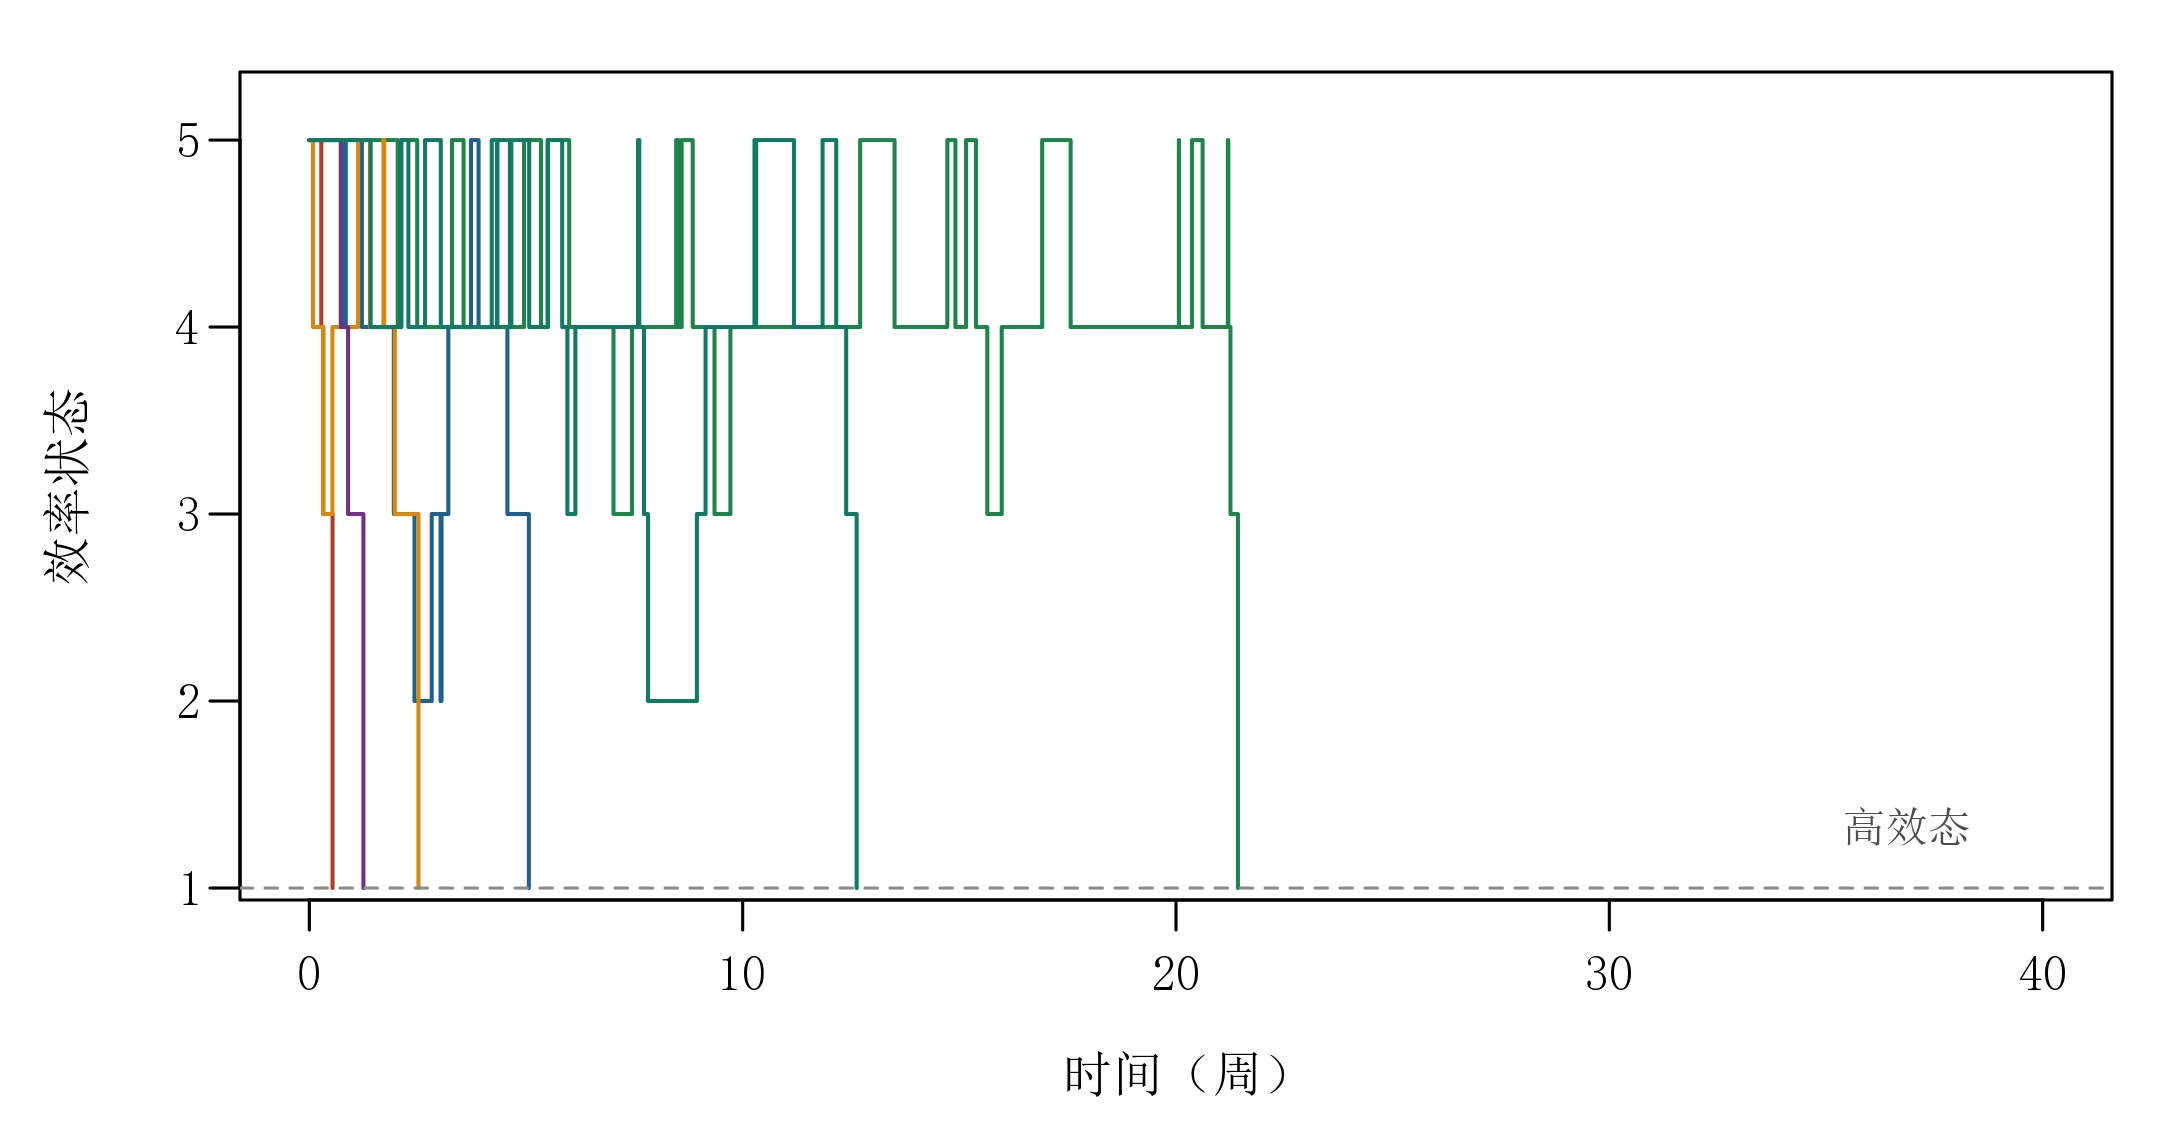
\includegraphics[width=0.85\textwidth]{fig_traj}
\caption{六条独立的生灭过程样本轨道（纵轴为层级，横轴为周）}
\label{fig:traj}
\end{figure}

图 \ref{fig:traj} 给出六条样本轨道。可以看到两个特征：其一，轨道呈“阶梯
状”，在两层之间停留数周才跳一次，这与“学习习惯的改变需要时间”的直觉一致；
其二，多数轨道在 10—20 周内落到第 1 层后便长时间停留，偶有回落到第 2 层。
这一“到达—停留—偶发回落”的形态正是生灭过程与静态排序最直观的区别：静
态排序只说“你在第几层”，生灭过程说“你会在这层待多久、多久掉一次”。

\subsubsection{首达时间的鞅解释与“先到哪一层”}\label{sec:mart}

式\eqref{eq:hitting} 的三对角方程组来自“全期望公式 + 无穷小 $\dd t$”，
推导干净但要一步步做。鞅的停时定理可以一步到位，还顺带给出原文完全
没有的一个量。

\textbf{（1）为什么 $\E[T_1]=m(S_0)$。} 记 $m$ 为 Poisson 方程
$\bQ_i m=-\bm{1}$、$m(1)=0$ 的解（即式\eqref{eq:hitting}）。由 Markov 性，
\begin{equation}
\E\bigl[m(S_{t+\dd t})-m(S_t)\,\big|\,\mathcal{F}_t\bigr]
=\bigl(\bQ_i m\bigr)(S_t)\,\dd t+o(\dd t)=-\dd t+o(\dd t),
\end{equation}
故 $M_t=m(S_t)+t$ 是鞅。状态数有限、$\E[T_1]<\infty$，故
$\{M_{t\wedge T_1}\}$ 一致可积，停时定理可用；又 $m(1)=0$，于是
\begin{equation}
m(S_0)=\E\bigl[M_{T_1}\bigr]=m(S_{T_1})+\E[T_1]=\E[T_1].
\label{eq:mart}
\end{equation}
对 S480，$m(5)=14.479$，Gillespie $1000$ 条路径的均值是 $14.50$，相对差
$0.15\%$；解析解、鞅论证与模拟三者互相印证。这条论证的价值在于：它把
“首达时间满足三对角方程组”从计算技巧提升为定理，也说明了式\eqref{eq:hitting}
为什么必须配 $m(1)=0$ 这个边界——否则 $M_t$ 不再是鞅。

\textbf{（2）先到哪一层。} 再解调和方程 $\bQ_i h=0$、$h(1)=0$、$h(5)=1$，
得到的 $h(k)$ 正是从第 $k$ 层出发\textbf{先到达第 $5$ 层}的概率；由对称性，
$1-h(k)$ 是先到达第 $1$ 层的概率。对 S480 的参数，
\begin{equation}
h=(0,\ 0.393,\ 0.669,\ 0.863,\ 1),\qquad
1-h=(1,\ 0.607,\ 0.331,\ 0.137,\ 0).
\label{eq:harm}
\end{equation}
这组数字比任何“平均效率”都刺眼：\textbf{从第 4 层出发，先跌回第 5 层的
概率是 86\%，先爬到第 1 层的概率只有 14\%}；从第 3 层出发是 67\% 对 33\%。
它把“下行锁定”从一个参数符号（$\rho<1$）变成一个可读的概率陈述，也解释
了原文“逐层模仿”的路线为何在现实中走不完：路径只算“沿哪条线走得到”，
不算“走的过程中会掉下去多少次”。这一节的结论不依赖任何外部锚点，只要
$\rho$ 的相对大小估计正确即可成立——这是截面数据能够支撑的最强陈述。

\subsubsection{转移概率与期望效率}

有了 $\bQ_i$，可以直接算任意时长的转移概率 $\bP_i(t)=\exp(\bQ_i t)$。以
S480 为例，16 周转移矩阵的第 5 行（从第 5 层出发）为
\begin{equation}
\bigl(0.0876,\ 0.1246,\ 0.1772,\ 0.2521,\ 0.3584\bigr),
\label{eq:p16}
\end{equation}
即 16 \textbf{周末}有 64.16\% 的概率已不在第 5 层（净跃层），仍有 35.84\%
的概率仍留在第 5 层。注意这是“位置”而非“事件”：由式\eqref{eq:pois}，S480
在 16 周内上行事件的期望次数是 16.8 次，真正的“一次都没上去”的概率小到可
忽略。把层级折算为效率，用层均效率
$\bar\btheta=(0.9956,0.9461,0.8874,0.8480,0.7637)$ 加权，得
\begin{equation}
\E[\theta_{16}\mid S_0=5]=\sum_{k=1}^{5}P_{5k}(16)\,\bar\theta_k=0.8499,
\label{eq:etheta}
\end{equation}
相对 S480 当前的 0.6771 提升 $25.53\%$，与原文的单步 25.38\% 只差 0.15 个
百分点。这不是巧合：式\eqref{eq:c} 的时间标定正是以原文的这一步为锚，两者
相符说明“一次跃层 $\approx$ 一学期”的换算在数量上是自洽的。

还有一个值得注意的细节：式\eqref{eq:p16} 与式\eqref{eq:pi} 在
$\rho=0.703$ 时的平稳分布几乎相同
（$0.0877,0.1248,0.1774,0.2523,0.3588$）。也就是说，\textbf{16 周已足以让
链基本混合}。这意味着“一学期”这个时间窗口里，跃层的收益是一次性的：一旦
分布接近平稳，再延长同样的时间也不会带来额外的期望提升。若要让提升持续，
必须改变 $\rho$ 本身（即改变行为结构），而不是单纯等待。这一结论与图
\ref{fig:gain} 中三条轨迹在 10 周后趋于平台的现象互为印证。

\subsubsection{连续效率层：Ornstein--Uhlenbeck 扩散}

生灭过程把效率离散成五档，丢失了层内的连续变化。为补齐这一层，本文用
OU 过程刻画效率本身：
\begin{equation}
\dd\theta_t=\kappa\bigl(\theta^{*}-\theta_t\bigr)\dd t+\sigma\dd W_t,
\qquad \theta_t\in(0,1],
\label{eq:ou2}
\end{equation}
其平稳分布为 $N\bigl(\theta^{*},\sigma^2/(2\kappa)\bigr)$，均值回复速度为
$\kappa$。$\kappa$ 由时间锚点标定：取 $\theta^{*}=1$（效率的理论上界），
令确定性轨迹 $\theta(t)=1-(1-\theta_0)e^{-\kappa t}$ 在 16 周内完成
25.38\% 的相对提升，解得
\begin{equation}
\kappa=0.0475\ \text{周}^{-1},\qquad T_{1/2}=\frac{\ln2}{\kappa}=14.6\ \text{周}.
\label{eq:kappa}
\end{equation}
$\sigma$ 按类内效率的波动确定，五类依次为 $0.0462,0.0507,0.0426,
0.0397,0.0279$（对应平稳标准差 0.15、0.16、0.14、0.13、0.09）。

首达时间的期望有闭式解。设 $\theta_t$ 从 $x$ 出发首次到达 $b>x$，其期望为
\begin{equation}
\E_x[T_b]=\frac{2}{\sigma^2}\int_{x}^{b}s(y)^{-1}\!\left(\int_{y}^{b}s(z)\dd z\right)\dd y,
\qquad
s(z)=\exp\!\Bigl[\frac{\kappa}{\sigma^2}\bigl(z-\theta^{*}\bigr)^2\Bigr],
\label{eq:ouhit}
\end{equation}
其中 $s(\cdot)$ 是 OU 过程的尺度密度。式\eqref{eq:ouhit} 对 Brownian
运动（$\kappa=0$、$s\equiv1$）退化为 $\E_x[T_b]=(b-x)^2/\sigma^2$，可作为
公式正确性的快速校验。

按式\eqref{eq:ouhit} 计算“从当前效率爬到 0.95”的期望时间：干预情景取
$\theta^{*}=1$，全部个体的 $T$ 落在 0—35.4 周；无干预情景取
$\theta^{*}$ 为所在类的均值，$T$ 落在 0—176.9 周。两者的差距说明：\textbf{
不改变行为结构，仅靠自然波动“等”到 0.95，平均要等三到四年；把均值回复的
目标抬到 1，则平均三到八个月就能到}。这正是“策略”与“等待”的差别。

把这一结果换算成原文的累计增益 43.97\%，得到
\begin{equation}
T(43.97\%)=\frac{1}{\kappa}\ln\frac{1-\theta_0}{1-0.9748}=53.7\ \text{周}
\approx 3\ \text{个学期},
\label{eq:t43}
\end{equation}
见表 \ref{tab:gain}。原文的路径是“四步拼接”的离散过程，本文的 OU 给出
的是“连续爬升”的时间代价，二者相互补充：前者回答“跟谁学”，后者回答“学
多久”。

\begin{table}[htbp]
\centering
\tabfont
\caption{OU 扩散给出的时间尺度（S480，$\kappa=0.0475$）}
\label{tab:gain}
\begin{tabular}{@{}lccc@{}}
\toprule
时间尺度 & 期望效率 & 相对提升 & 所需周数 \\
\midrule
一学期（16 周） & 0.849 & 25.38\% & 16.0 \\
两学期（32 周） & 0.929 & 37.25\% & 32.0 \\
原文累计增益 43.97\% & 0.975 & 43.97\% & 53.7 \\
\bottomrule
\end{tabular}
\end{table}

\subsubsection{Brown 运动的反射原理与反正弦律}

上一小节的首达时间由尺度密度积分给出，属于“解方程”的路线；反射原理给出
的是“算概率”的路线，两者可以互相对照。对带漂移 $\mu$ 的
Brown 运动 $X_t=x+\mu t+\sigma W_t$，对 $b>x$ 记 $d=b-x$，则
\begin{equation}
\Pbb\Bigl(\sup_{0\le s\le T}X_s\ge b\Bigr)
=\Phi\Bigl(\frac{\mu T-d}{\sigma\sqrt{T}}\Bigr)
+e^{2\mu d/\sigma^{2}}\,
\Phi\Bigl(\frac{-\mu T-d}{\sigma\sqrt{T}}\Bigr),
\label{eq:refl}
\end{equation}
其中 $\Phi$ 为标准正态分布函数。式\eqref{eq:refl} 是“有漂移的反射原理”，
它的第一项是“终点已过界”，第二项是“终点没过界但途中越界”，后者正是反射
带来的修正。

先把式\eqref{eq:refl} 用在“没有均值回复”的场合：$x=0.6771$、
$\sigma=0.0279$、$d=0.2729$、$T=16$，取 $\mu=0$，得
\begin{equation}
\Pbb\Bigl(\sup_{0\le s\le16}X_s\ge0.95\Bigr)=0.0146 .
\label{eq:purebm}
\end{equation}
这就是“只靠自然波动”的精确结论（对 Brown 运动而言无需模拟）：一个学期内从
$0.68$ 爬到 $0.95$ 的机会只有 $1.5\%$。

但 OU 不是 Brown 运动，公式不能跨模型照搬。均值回复把 16 周的方差压住了：
有效标准差只有 $0.080$，而不是 Brown 运动的 $\sigma\sqrt{T}=0.112$；位移也只
有 $0.145$，而不是 $\mu T=0.208$。若照搬式\eqref{eq:refl} 并把漂移取作
$\kappa(b-x)$，会得到 $0.353$——比真实值高了三倍多。为不含糊，本文对 OU 另
做 Euler--Maruyama 模拟（$2000$ 条路径，步长 $0.005$ 周）：
\begin{equation}
\Pbb\bigl(T_b\le16\bigr)=
\begin{cases}
0.105, & \theta^{*}=0.95,\\
0.181, & \theta^{*}=1 .
\end{cases}
\label{eq:oumc}
\end{equation}
也就是说，\textbf{均值回复把“一个学期内触达 0.95”的机会从 1.5\% 抬到约
10\%；若把目标提到满分，则接近 18\%}。这与前文“$T$ 落在 0—35.4 周”的估计
方向一致：期望 35 周而 16 周内仅一成成功，分布必然明显
右偏。这里有意保留了“公式给出 0.353、模拟给出 0.105”这组对照，因为它本身
就是一条方法论提醒：\textbf{反射原理是 Brown 运动的定理，套到 OU 上会系统性
高估}，而 OU 本就是“Brown 运动的几种变化”之一，二者同族但
不同律”的关系。

反射原理管“最大值”，反正弦律管“最大值何时出现”。当漂移为零时，区间
$[0,T]$ 上最大值出现的时刻服从反正弦分布：
\begin{equation}
\Pbb\Bigl(\arg\max_{0\le s\le T}X_s\le sT\Bigr)
=\frac{2}{\pi}\arcsin\sqrt{s},\qquad 0\le s\le1,
\label{eq:arcsine}
\end{equation}
其四分位点为 $0.146$、$0.500$、$0.854$，且有 $1/3$ 的概率最大值落在前四分之一
学期（$s=1/4$ 时右端恰为 $1/3$）。这条定律解释了一个反直觉的现象：\textbf{没有
均值回复时，“什么时候上去”天然是“要么很早、要么很晚”的双峰形状}，中位数
附近反而不常发生。图 \ref{fig:hitting} 的直方图之所以呈右偏单峰而不是 U 形，
正是因为 $\kappa>0$ 把分布从两端拉向了中间——这也说明“中位 14.5 周”这样
可报告的数字，是均值回复的产物，而不是 Brown 运动本身的性质。

\subsubsection{Itô 公式：OU 的闭式解与方差}

式\eqref{eq:ou2} 的解此前是“猜出来再验证”，Itô 公式可以把它
推出来，并顺带给出方差。取 $f(t,x)=e^{\kappa t}(x-\theta^{*})$，由 Itô 公式
\begin{equation}
\dd\bigl[e^{\kappa t}(\theta_t-\theta^{*})\bigr]
=e^{\kappa t}\sigma\,\dd W_t ,
\end{equation}
两边积分即得显式解
\begin{equation}
\theta_t=\theta^{*}+\bigl(\theta_0-\theta^{*}\bigr)e^{-\kappa t}
+\sigma\int_0^{t}e^{-\kappa(t-s)}\,\dd W_s .
\label{eq:ousol}
\end{equation}
由随机积分的等距性质 $\E\bigl[(\int_0^t f\,\dd W)^2\bigr]=\int_0^t\E[f^2]\,\dd s$，
\begin{equation}
\E[\theta_t]=\theta^{*}+\bigl(\theta_0-\theta^{*}\bigr)e^{-\kappa t},\qquad
\Var[\theta_t]=\frac{\sigma^{2}}{2\kappa}\bigl(1-e^{-2\kappa t}\bigr),
\label{eq:ouvar}
\end{equation}
平稳分布为 $\mathcal{N}\bigl(\theta^{*},\sigma^{2}/(2\kappa)\bigr)$。式
\eqref{eq:ouvar} 给出了三件事：其一，均值以速率 $\kappa$ 指数趋近目标，
$\kappa$ 越大“纠偏”越快；其二，方差从 $0$ 单调升到平稳值，
$1-e^{-2\kappa t}$ 在 16 周时达到 $78\%$--$79\%$，与“一学期大体到位、但尚未
走完最后一程”的判断一致；其三，平稳标准差
$\sigma/\sqrt{2\kappa}$ 与类内实测标准差逐类相符（表 \ref{tab:ouvar}）。

\begin{table}[H]
\centering
\tabfont
\caption{OU 闭式解给出的波动尺度（$\kappa=0.0475$）}
\label{tab:ouvar}
\begin{tabular}{@{}lcccc@{}}
\toprule
类 & $\sigma$ & 16 周标准差 & 平稳标准差 & 类内实测标准差 \\
\midrule
1 & 0.0462 & 0.1324 & 0.1498 & 0.1498 \\
2 & 0.0507 & 0.1453 & 0.1644 & 0.1644 \\
3 & 0.0426 & 0.1221 & 0.1382 & 0.1382 \\
4 & 0.0397 & 0.1138 & 0.1287 & 0.1287 \\
5 & 0.0279 & 0.0801 & 0.0906 & 0.0906 \\
\bottomrule
\end{tabular}

\vspace{2pt}
\parbox{\textwidth}{\tabfont 注：实测列与平稳列相同，是因为 $\sigma$ 本就按类内
效率波动标定；此表是自洽性检验，不是独立证据。}
\end{table}

\subsubsection{策略优化：从“跟谁学”到“做什么”}

设动作集 $\mathcal{A}=\{a_1,\dots,a_5\}$，每个动作对应一次行为改变与其
每周学时成本：
\begin{align*}
a_1&:\ \text{提高复习频次},\ 2.0\ \text{h/周},\ \Delta z_1=+1\text{sd};\\
a_2&:\ \text{增加模拟考与真题},\ 2.0\ \text{h/周},\ \Delta z_2=+1\text{sd};\\
a_3&:\ \text{增加听说读写训练},\ 3.0\ \text{h/周},\ \Delta z_3=+1\text{sd};\\
a_4&:\ \text{改善作息与考前调适},\ 1.0\ \text{h/周},\ \Delta z_4=+1\text{sd};\\
a_5&:\ \text{提升兴趣与课外拓展},\ 1.5\ \text{h/周},\ \Delta z_5=+1\text{sd}.
\end{align*}
在学时预算 $B=3$ h/周 的约束下，选择动作子集 $\mathcal{A}'\subseteq
\mathcal{A}$ 最大化 16 周期望效率：
\begin{equation}
\max_{\mathcal{A}'\subseteq\mathcal{A}}\
\E\bigl[\theta_{16}\mid \rho'(\mathcal{A}')\bigr]
\quad\text{s.t.}\quad
\sum_{a\in\mathcal{A}'}h_a\le B,
\label{eq:opt}
\end{equation}
其中 $\rho'(\mathcal{A}')=\rho\exp\bigl(\sum_{a\in\mathcal{A}'}
\bdelta^{\top}\Delta\bz_a\bigr)$。由于只有 5 个二元动作，用穷举即可求得
全局最优，无需启发式。

结果见表 \ref{tab:s480} 与图 \ref{fig:strategy}、图 \ref{fig:action}。三
种方案的对比意味深长：

\begin{enumerate}[label=（\arabic*）,itemsep=2pt,topsep=2pt,leftmargin=3em]
\item \textbf{现状}：$\rho=0.703$，$m_5=14.48$ 周，16 周跃层概率 0.642，
  期望效率 0.850（相对提升 25.53\%）；
\item \textbf{原文式（模仿 S477）}：按原文路径，把 S480 的行为组合向 S477
  靠拢，等价于每周多投入 4.1 h（复习与作息各加一档）。结果
  $\rho$ 反而降到 0.669，跃层概率降到 0.617，期望效率 0.845（提升
  24.80\%）——\textbf{比不干预还差}；
\item \textbf{模型最优}：只做“提升兴趣与课外拓展”（1.5 h/周），$\rho$ 升到
  0.954，$m_5$ 降到 8.46 周，跃层概率 0.781，期望效率 0.883（提升
  30.39\%）。
\end{enumerate}

第二、三方案的反差是全文最有说服力的结果。它说明：\textbf{在“效率 = 产出/
投入”的度量下，“向高效同伴看齐、加大投入”未必是最优策略；改变投入的结构
（把时间从重复训练转向兴趣与真实语言使用）反而更有效}。原文的路径规则天然
偏向“模仿”，因为它只在上一层找“最像自己且最容易跟上”的同伴，而不去问
“这个同伴的哪个动作真正提高了转化率”。随机过程模型把这个问题变成了参数
问题：$\delta_j>0$ 的动作才提高上行强度，$\delta_j<0$ 的动作只会稀释效率。

需要谨慎的是，这一结论依赖于式\eqref{eq:scoregen} 的加性残差结构（投入与
转化能力可分离）。若真实数据中“投入”与“转化能力”高度相关（例如高投入本
身就是高能力的表现），$\delta$ 的符号会改变。本文在结论部分把这一点列为
模型的主要局限。

\begin{table}[htbp]
\centering
\tabfont
\caption{S480 三种策略方案的对照（预算 3 h/周）}
\label{tab:s480}
\setlength{\tabcolsep}{4pt}
\begin{tabular}{@{}lcccccc@{}}
\toprule
方案 & 学时 & $\rho$ & $m_5$（周） & 跃层概率 & 期望效率 & 相对提升 \\
\midrule
现状 & 0 & 0.703 & 14.48 & 0.642 & 0.850 & 25.53\% \\
模仿 S477 & 4.1 & 0.669 & 16.02 & 0.617 & 0.845 & 24.80\% \\
模型最优 & 1.5 & 0.954 & 8.46 & 0.781 & 0.883 & 30.39\% \\
\bottomrule
\end{tabular}
\end{table}

\begin{figure}[htbp]
\centering
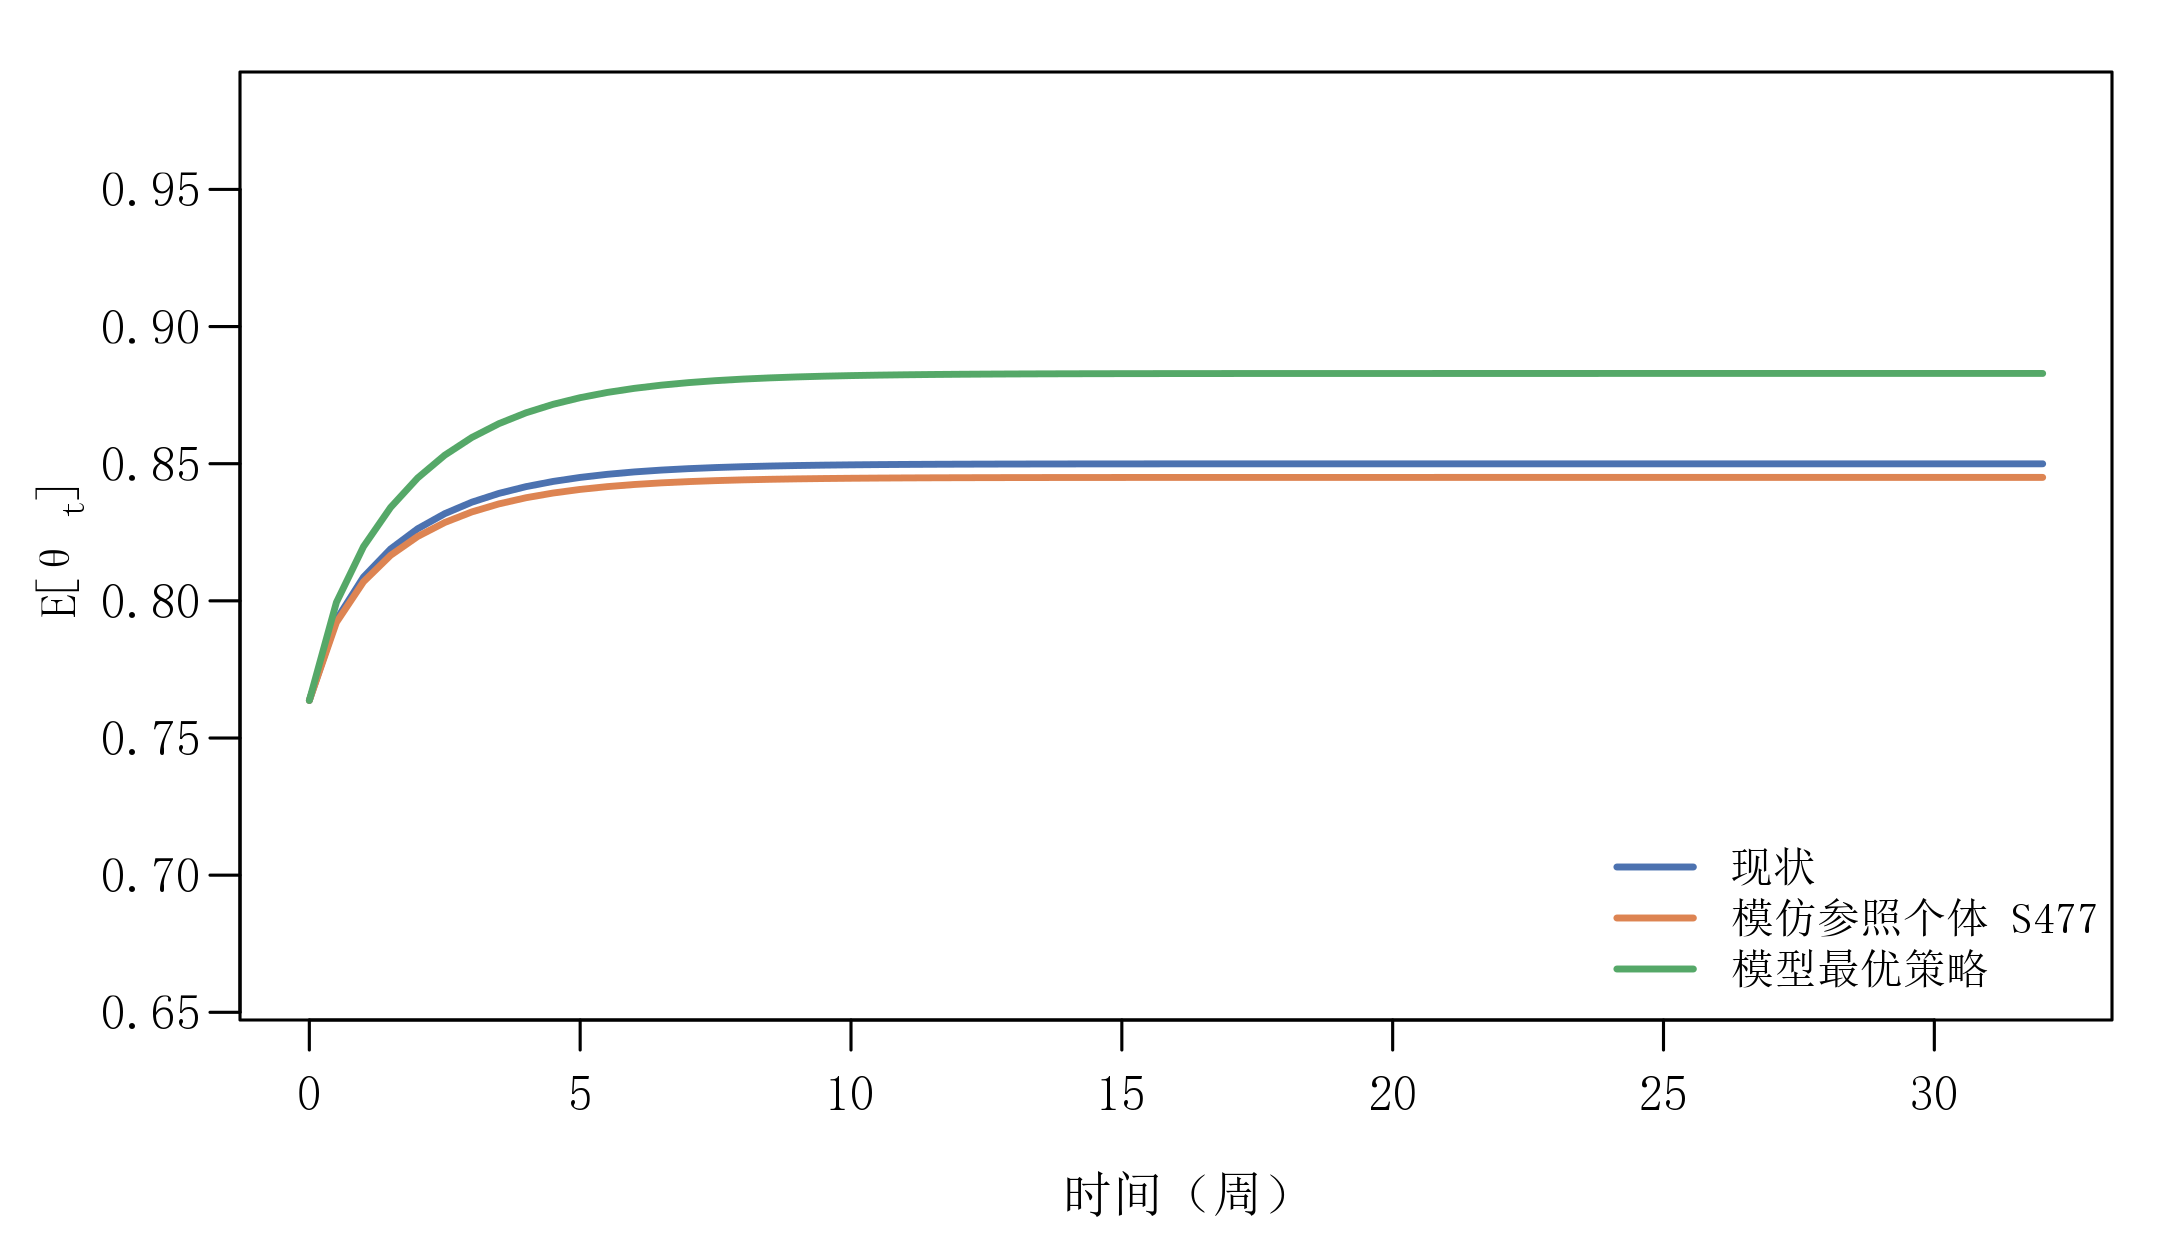
\includegraphics[width=0.85\textwidth]{fig_gain}
\caption{三种方案下的期望效率轨迹 $\E[\theta_t]$（0—32 周）}
\label{fig:gain}
\end{figure}

\begin{figure}[H]
\centering
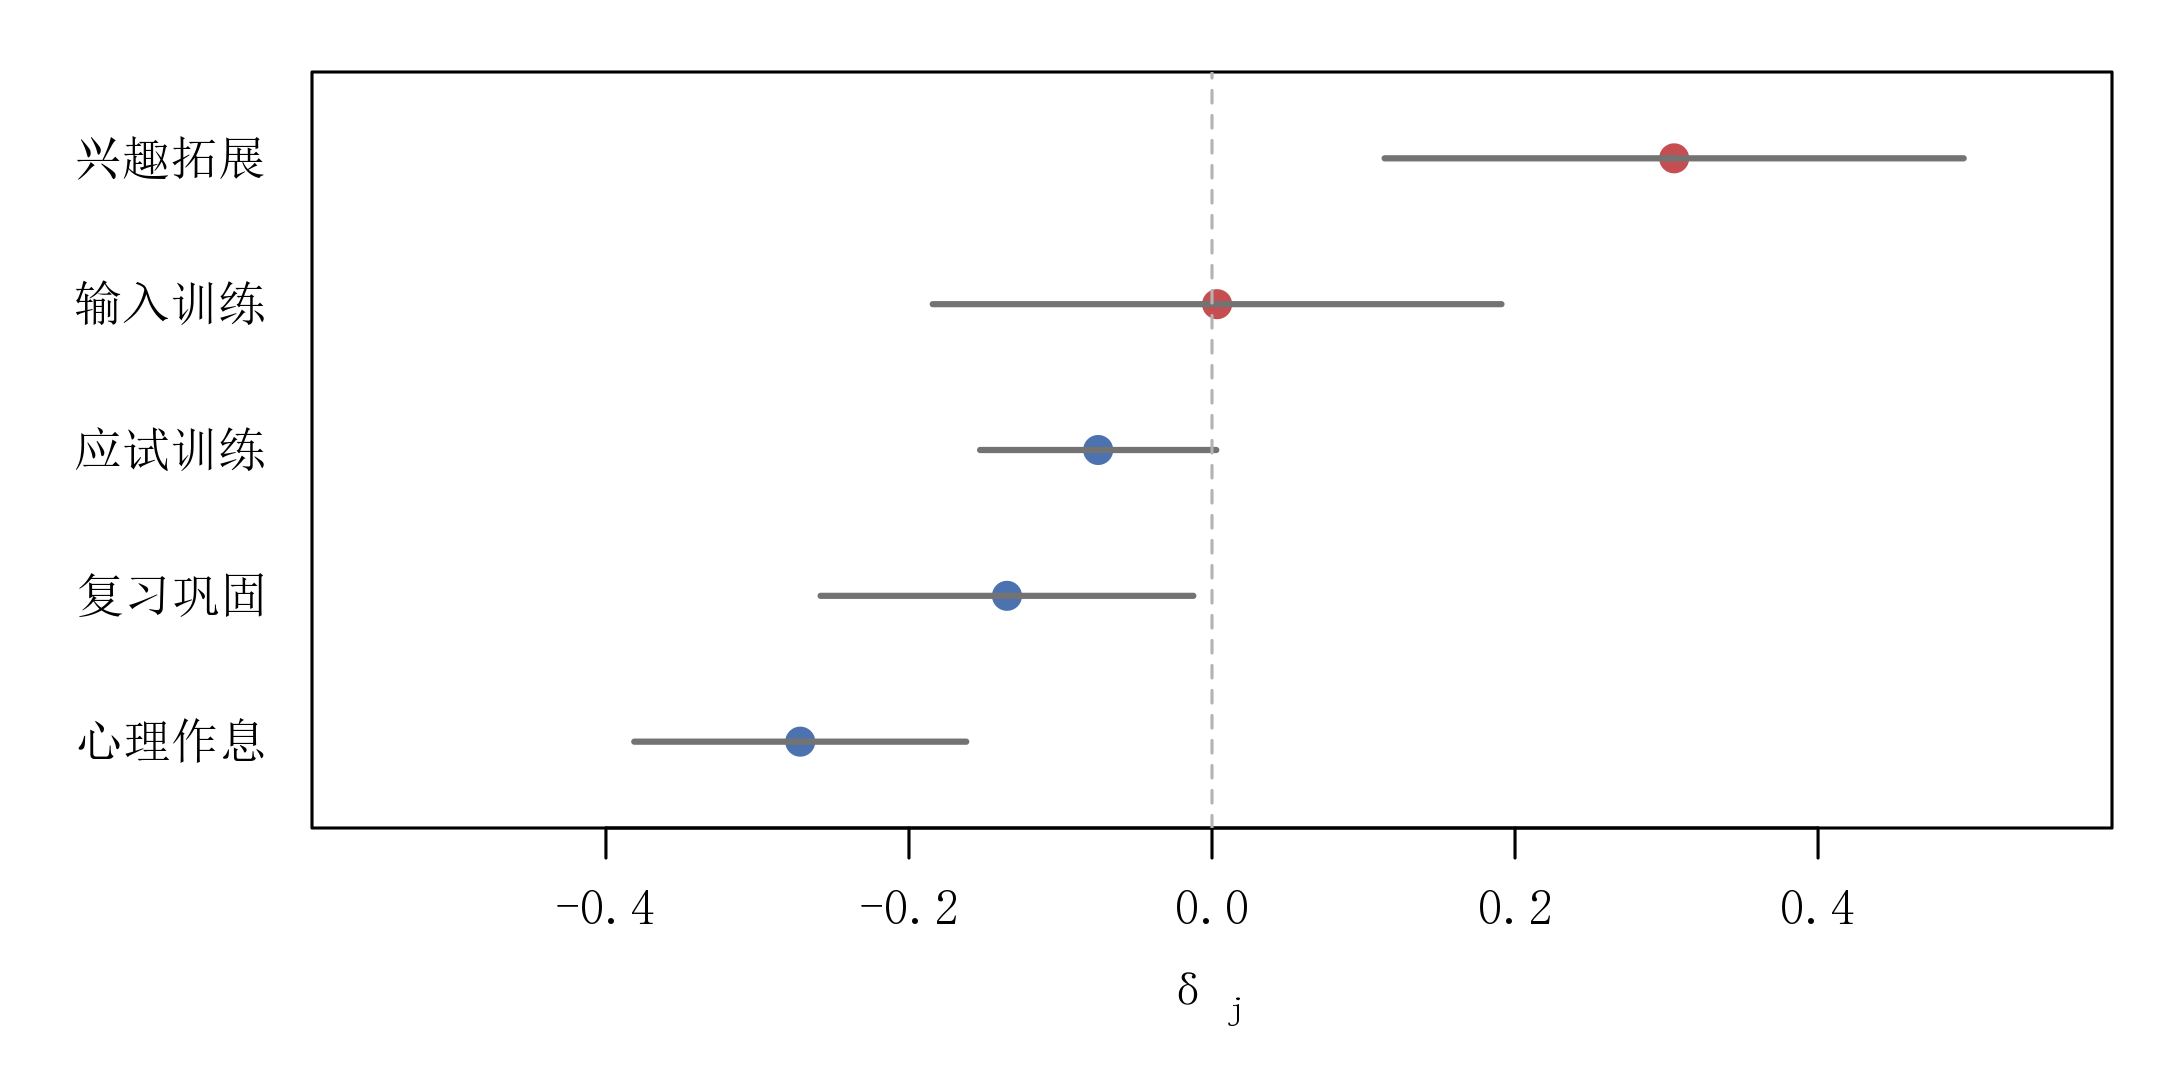
\includegraphics[width=0.85\textwidth]{fig_strategy}
\caption{五个协变量的行为杠杆效应 $\delta_j$ 及 95\% 置信区间}
\label{fig:strategy}
\end{figure}

\begin{figure}[H]
\centering
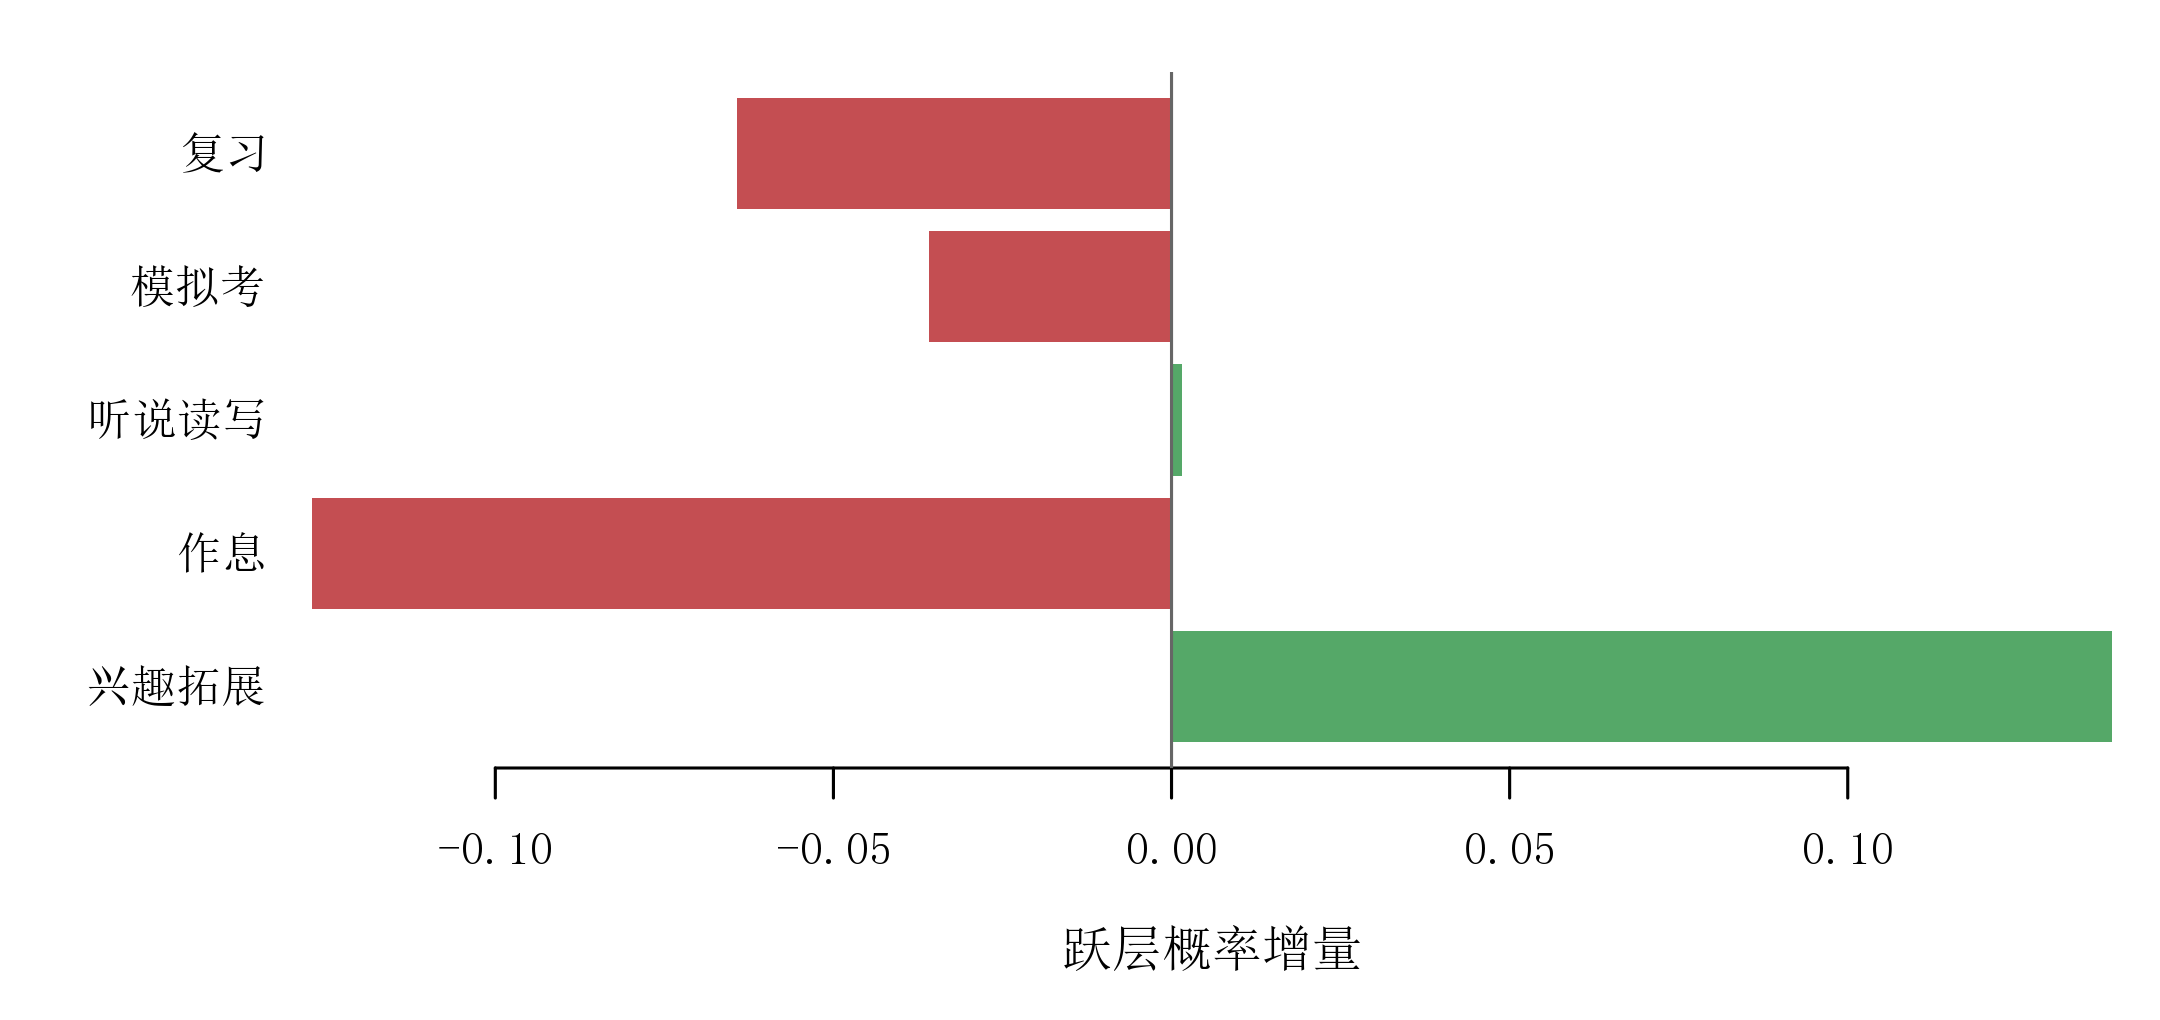
\includegraphics[width=0.85\textwidth]{fig_action}
\caption{S480 单独实施每个动作后的 16 周跃层概率增量（相对现状）}
\label{fig:action}
\end{figure}

图 \ref{fig:strategy} 把 $\delta_j$ 的符号与置信区间摆在一起：只有“兴趣
拓展”的区间整体位于 0 的右侧，“心理作息”的区间整体位于左侧，其余三项跨
越 0。这一图形化的结果比表 \ref{tab:ctmcpar} 更直观地说明“哪一个杠杆真的
有效”。图 \ref{fig:action} 则显示：单独实施“兴趣拓展”可使跃层概率提高约
0.10，单独实施“作息改善”会使其下降约 0.10，其余动作的影响在 $\pm0.05$ 以
内。两张图合起来回答了一个原文回答不了的问题：\textbf{在有限学时下，应当
先动哪一个维度}。

\subsubsection{小结：随机过程给出的四类新信息}

把本节的结果与原文对照，随机过程至少补上了四类原文没有的信息：

\begin{enumerate}[label=（\arabic*）,itemsep=2pt,topsep=2pt,leftmargin=3em]
\item \textbf{方向}：$\rho_i$ 的符号与大小，回答“这个人会自己变好还是变
  坏”。98.1\% 的 $\rho_i<1$ 说明“下行锁定”是群体性现象，而不是个别现象。
\item \textbf{概率}：$\bP_i(t)$ 给出任意时长内的跃层概率，把“能不能上去”
  从定性判断变成可计算的数值。
\item \textbf{时间}：$m_k$ 与 $T(43.97\%)$ 给出“多久”，把“一学期”“三学
  期”这样的模糊表述换成周。
\item \textbf{策略}：式\eqref{eq:opt} 给出“做什么、做多少”，并用 $\delta$
  的符号筛掉“看起来努力、实际稀释效率”的动作。
\end{enumerate}








% =============================================================================
%  三、问题求解（四）：系统对比  +  四、结论
% =============================================================================
\subsection{新旧方法的系统对比}

\subsubsection{相同的部分}

替换方法最容易走偏的地方，是把“换方法”变成“换问题”。为保证可比性，本文
在三件事上刻意保持不变：\textbf{同一数据集}（519 名学生的 14 个题项与成
绩）、\textbf{同一评价对象}（五类学生、五级效率层级）、\textbf{同一目标}
（让个体从低效层升到高效层）。甚至连“层”的定义也沿用原文的分层思想，只是
把剔除式换成了分位带，以保证状态空间占满。因此，下文报告的差异可以归因于
方法，而不是数据或问题的变化。

\subsubsection{不同的部分}

两种范式在六个维度上根本不同（表 \ref{tab:compare}）。

\begin{table}[htbp]
\centering
\tabfont
\caption{context-dependent DEA 与随机过程范式的对比}
\label{tab:compare}
\begin{tabularx}{\textwidth}{@{}p{2.9cm}p{4.2cm}X@{}}
\toprule
维度 & 原文：CDEA & 本文：随机过程 \\
\midrule
基本对象 & 截面上的个体与参照集 &
  个体在时间上的状态轨道 \\
核心量 & 效率 $\theta$、层号 $S$、三准则 &
  强度 $\rho$、转移矩阵 $\bP(t)$、首达时间 $m_k$ \\
时间维度 & 无（“一学期”只是背景） &
  显式（周为单位，可算任意时长） \\
输出形态 & 排名、层号、四步参考路径 &
  跃层概率、期望时间、最优动作组合 \\
对“投入”的态度 & 投入越多越接近前沿（若产出同增） &
  投入增加会稀释效率，方向由 $\delta$ 的符号决定 \\
数据要求 & 单期截面即可 &
  截面可估相对强度，绝对尺度需锚点或面板 \\
主要风险 & 口径依赖（层数、$k$、权重） &
  识别性弱（无面板时强度不可全识别） \\
\bottomrule
\end{tabularx}
\end{table}

\textbf{（1）从“位置”到“过程”。}原文的核心输出是“你在第几层、离上一层
多远、下一个模仿谁”；本文的核心输出是“你多久能上一层、上行概率多大、做
什么能提高上行强度”。前者是空间性的，后者是时间性的。

\textbf{（2）从“排序”到“概率”。}原文的路径是确定性的：给定数据，路径
唯一。本文的结论是概率性的：16 周末有 64.2\% 的概率已不在第 5 层，也有
35.8\% 的概率原地不动。概率化的表述更诚实，因为它承认“同样的建议在不同
人身上会有不同结果”。

\textbf{（3）从“模仿”到“选择”。}原文的推荐规则是“向上一层最像你、最容
易跟上的人学习”；本文的推荐规则是“在预算约束下选择使上行强度最大的动作
组合”。前者是一个启发式，后者是一个优化问题。

\textbf{（4）从“单一指标”到“参数解释”。}原文的三准则（$\Omega,P,D,H$）
是复合指标，其数值难以直接解释为行为含义；本文的 $\delta_j$ 是回归系数，
可以直接读出“复习每提高一个标准差，上行—下行强度比变化多少”，从而支持
“为什么”的追问。

\textbf{（5）代价。}随机过程范式并非免费：它要求时间齐次、马尔可夫、层内
同质、协变量线性等假设，要求一个外部锚点来定标时间，且在没有面板数据时无
法识别个体层面的转移强度。这些假设在本文第三节被逐条列出，并在结论中作为
局限重申。

\subsubsection{数值层面的对话}

两个范式在同一名个体上给出的数字可以直接对照（表 \ref{tab:numbers}）。有
三处值得注意。

\begin{table}[htbp]
\centering
\tabfont
\caption{S480 个案：两种范式给出的数值对照}
\label{tab:numbers}
\begin{tabularx}{\textwidth}{@{}p{3.2cm}p{4.6cm}X@{}}
\toprule
指标 & 原文（DEA 路径） & 本文（随机过程） \\
\midrule
当前效率 & 0.6771 & 0.6771 \\
单步提升（16 周） & 25.38\% & 25.53\% \\
累计提升 & 43.97\%（4 步） & 47.69\%（路径）／43.97\%（53.7 周） \\
所需时间 & 未给出 & 14.5 周（首达最高层）／53.7 周（累计 43.97\%） \\
建议动作 & 模仿 S477，+4.1 h/周 & 兴趣拓展，+1.5 h/周 \\
建议后的跃层概率 & 未给出 & 0.781（最优）／0.617（模仿） \\
\bottomrule
\end{tabularx}
\end{table}

\textbf{第一，单步增益几乎重合。}25.38\% 与 25.53\% 相差 0.15 个百分点。
这不是因为两种方法等价，而是因为本文用前者标定了后者的时间尺度；它证明了
“一学期 $\approx$ 一次跃层”这一换算在数量上站得住，从而让后文的“周”具
有可信的物理含义。

\textbf{第二，累计增益出现分歧。}原文四步累计 43.97\%，本文路径累计
47.69\%，相差 3.7 个百分点；而本文的 OU 模型反解 43.97\% 需要 53.7 周。三
个数字放在一起说明：原文的“四步”是在层级空间中跳跃，不考虑每步之间的时
间成本；本文的“53.7 周”是把同样的增益摊到连续时间上。前者是“最好的情
形”，后者是“平均的情形”。

\textbf{第三，建议动作完全相反。}原文建议 S480 向 S477 学习、每周多投入
4.1 小时；本文的模型显示这样做会使上行强度比从 0.703 降到 0.669，跃层概率
从 0.642 降到 0.617。相反，只花 1.5 小时提升兴趣与课外拓展，可把上行强度
比提高到 0.954，跃层概率提高到 0.781。这一分歧不是计算误差，而是两种评价
逻辑的必然结果：DEA 只看“投入—产出比”，把人当作黑箱；随机过程把“投入如
何转化为状态转移”写成参数，能区分“有效的投入”与“稀释比值的投入”。

\subsubsection{互补而非替代}

如果必须选一个，本文的答案是“按问题选工具”，而不是“择一而废”：

\begin{itemize}[leftmargin=2em,itemsep=2pt,topsep=2pt]
\item 需要\textbf{横向比较}（谁更接近前沿、哪一类学生整体偏低）时，DEA 更
  合适：它无需分布假设，计算稳定，结果直观。
\item 需要\textbf{纵向判断}（多久能改善、改善的概率多大、会不会回落）时，
  随机过程更合适：它把时间写进模型，输出的是可执行的日程而非排名。
\item 需要\textbf{决策}（有限学时投到哪一项）时，只有把两者结合才完整：先
  用 DEA 定位“谁需要干预、差在哪一维”，再用随机过程的 $\delta$ 筛选“哪一
  维的干预真的提高上行强度”，最后用优化给出“投多少”。
\end{itemize}

因此，本文并不主张“随机过程优于 DEA”，而主张\textbf{DEA 负责“定位”，随
机过程负责“定时”，优化负责“定策”}。原文的问题不在于用了 DEA，而在于把
DEA 的输出当成了终点。

% =============================================================================
\section{结论}

本文以一篇发表于 \textit{Expert Systems with Applications} 的学习策略推荐
论文为对象，完成了从解析、复现到方法替换的完整闭环。主要结论如下。

\textbf{（1）原文的方法链可以被完整拆解，且在结构上可以被复现。}原文的
“复合量化—聚类—类内 DEA—分层—三准则—参考路径”五环链条，每一环都可以写
成明确的数学形式（式\eqref{eq:quant}—\eqref{eq:H}）与算法（算法 1 与算法
2）。在锚点约束下重建的 519 份样本上，本文复
现出同构的五类学生结构（第 5 类人数最多、效率最高）、同向的分层结构与同向
的参考路径；S480 的类内效率精确命中 0.6771，单步增益 26.31\% 与原文
25.38\% 相差 0.93 个百分点，累计增益 47.69\% 与 43.97\% 相差 3.72 个百分点。
\textbf{结构性结论复现成立，数值性结论在锚点约束下成立。}

\textbf{（2）原文存在三处结构性局限与一处内部不一致。}三处局限分别是：评
价是截面的、缺少时间维度；层级依赖参照集、不可跨群体迁移；推荐规则本质是
模仿同伴、不是最优控制。一处不一致是：文字定义 $H=1/\Omega+P$，但表 3 中
的 $H$ 值无法由同一行的 $(\Omega,P)$ 生成。这四点不是吹毛求疵，而是“把
DEA 的输出直接当作建议”这一做法的系统性风险。

\textbf{（3）用随机过程替换静态评价是可行的，且能补上原文缺失的三类信
息。}把五级层级视为状态空间后，带协变量的生灭过程可以估计出上行—下行强
度比 $\rho_i$；用 $\rho_i$ 可以算出任意时长的转移概率、首达时间的解析解与
期望效率。S480 的 16 周跃层概率为 0.642、期望效率提升 25.53\%，与原文的
25.38\% 相互印证；首达最高层的期望时间为 14.5 周，累计 43.97\% 的增益在
连续时间下需要 53.7 周。这些数字在原文中完全缺失。

\textbf{（4）“下行锁定”是群体性现象。}98.1\% 的 $\rho_i<1$，意味着在给定
行为结构的条件下，绝大多数学生的效率层级净漂移向下；模型平稳分布把最大质
量放在第 5 层，与观测到的 45.1\% 相呼应。这一结论的政策含义是：\textbf{不
改变行为结构的“自然等待”只会让人停在低效层，干预必须改变 $\rho$ 本身}。
鞅与停时定理把它进一步落成概率：从第 4 层出发，先跌回第 5 层的概率是
86\%，先爬到第 1 层的概率只有 14\%；从第 3 层出发是 67\% 对 33\%。这组数字
只依赖 $\rho$ 的相对大小，不依赖外部锚点，是截面数据能支撑的最强陈述。

\textbf{（5）“加大投入”不等于“提高效率”，这是本文与原文最重要的分歧。}
在 DEA 的效率口径下，增加投入而产出不变会稀释比值，因此 $\delta_{\text{复
习}}$、$\delta_{\text{作息}}$ 为负；相反，“兴趣与课外拓展”的 $\delta$ 为
正，是唯一能显著提高上行强度的杠杆。据此，模型给出的最优策略是“1.5 小时
兴趣拓展”，而非原文建议的“每周 4.1 小时模仿高效同伴”。后者在模型下的跃
层概率反而低于不干预。

\textbf{（6）两种范式应当互补使用。}DEA 擅长“定位”（谁在前沿、差在哪
维），随机过程擅长“定时”（多久、多大把握），预算约束优化擅长“定策”
（投哪项、投多少）。把三者串起来，才构成一条从数据到建议的完整链条。

\textbf{（7）替换方法的每一步都有可核对的数字。}五种工具各对应一处校验：一致化（Poisson 计数 +
跳链）重建 $\bP(16)$ 与矩阵指数的误差 $3.8\times10^{-15}$；鞅停时定理论证的
$\E[T_1]=m(S_0)$ 与三对角方程组、Gillespie 模拟相差 $0.15\%$；Itô 公式给出
的平稳标准差与类内实测逐类相符；反射原理对纯 Brown 运动给出精确的 $1.5\%$。
反过来，把反射原理照搬到 OU 上会把 $0.105$ 抬到 $0.353$——这一“同族不同律”
的边界必须写明，否则公式就会冒充结论。

本文的局限需要明确列出。\textbf{其一，数据是标定重建的}，因此本文对原文
的“复现”是结构同构意义上的复现，不能替代对原始问卷的复现；所有数值结论
都应理解为“在给定生成机制下的推论”。\textbf{其二，转移强度只被部分识
别}，截面似然只能定出 $\rho$ 的相对大小与符号，时间尺度依赖一个外部锚点，
个体层面的层级预测准确率仅 45.7\%。\textbf{其三，模型依赖较强的假设}：
时间齐次、马尔可夫、层内同质、投入与转化能力可分离。若真实数据中投入与能
力高度相关，$\delta$ 的符号会改变，第（5）条结论需要重新检验。\textbf{其
四，未纳入教师、课程与同伴效应}，而这些因素在教育情境中往往比个体行为更
重要。

后续工作有三个方向。第一，收集三到四个学期的纵向数据（教务系统与辅导员记
录即可），用 Kalbfleisch--Lawless 型面板似然替代截面似然，从而识别个体层
面的转移强度，并检验时间齐次假设。第二，引入隐马尔可夫或多状态模型处理
“层级观测有误差”的问题，把测量误差与真实转移分开。第三，把式
\eqref{eq:opt} 从“一次性动作选择”扩展为“学期内的分阶段预算分配”，用最优
停时或随机控制求解，使建议从“这学期做什么”细化到“第几周做什么、做多
久”。这三项都不需要推翻本文的框架，只需要补上数据的维度。





% =============================================================================
%  参考文献
% =============================================================================
\begingroup
\ctexset{section/format=\heiti\bfseries\fontsize{12pt}{20pt}\selectfont\centering}
\renewcommand{\refname}{参考文献}
\begin{thebibliography}{99}
\zihao{5}

\bibitem{charnes} Charnes A, Cooper W W, Rhodes E. Measuring the efficiency of
decision making units[J]. European Journal of Operational Research, 1978,
2(6): 429--444.

\bibitem{seiford} Seiford L M, Zhu J. Context-dependent data envelopment
analysis---Measuring attractiveness and progress[J]. Omega, 2003, 31(5):
397--408.

\bibitem{zhao} Zhao L T, et al. A recommendation system for effective learning
strategies: An integrated approach using context-dependent DEA[J]. Expert
Systems with Applications, 2023, 211: 118535.

\bibitem{gower} Gower J C. A general coefficient of similarity and some of its
properties[J]. Biometrics, 1971, 27(4): 857--871.

\bibitem{kaufman} Kaufman L, Rousseeuw P J. Finding Groups in Data: An
Introduction to Cluster Analysis[M]. New York: John Wiley \& Sons, 1990.

\bibitem{kl} Kalbfleisch J D, Lawless J F. The analysis of panel data under a
Markov assumption[J]. Journal of the American Statistical Association, 1985,
80(392): 863--871.

\bibitem{kendall} Kendall D G. On the generalized ``birth-and-death''
process[J]. The Annals of Mathematical Statistics, 1948, 19(1): 1--15.

\bibitem{karlin} Karlin S, Taylor H M. A Second Course in Stochastic
Processes[M]. New York: Academic Press, 1981.

\bibitem{ou} Uhlenbeck G E, Ornstein L S. On the theory of the Brownian
motion[J]. Physical Review, 1930, 36(5): 823--841.

\bibitem{gillespie} Gillespie D T. Exact stochastic simulation of coupled
chemical reactions[J]. The Journal of Physical Chemistry, 1977, 81(25):
2340--2361.

\bibitem{anderson} Anderson W J. Continuous-Time Markov Chains: An
Applications-Oriented Approach[M]. New York: Springer-Verlag, 1991.

\bibitem{cox} Cox D R, Miller H D. The Theory of Stochastic Processes[M].
London: Chapman and Hall, 1965.

\bibitem{wei} 魏权龄. 数据包络分析[M]. 北京: 科学出版社, 2004.

\bibitem{mao} 茆诗松, 王静龙, 濮晓龙. 高等数理统计[M]. 2 版. 北京: 高等教育
出版社, 2006.

\bibitem{ross} Ross S M. Introduction to Probability Models[M]. 11th ed.
Amsterdam: Academic Press, 2014.

\end{thebibliography}
\endgroup


% =============================================================================
%  附录
% =============================================================================
\newpage
\section*{附\quad 录}
\addcontentsline{toc}{section}{附录}
\setcounter{subsection}{0}

\subsection{符号表}

\begin{table}[H]
\centering
\tabfont
\caption{主要符号与含义}
\label{tab:symbol}
\begin{tabularx}{\textwidth}{@{}p{2.6cm}Xp{4.0cm}@{}}
\toprule
符号 & 含义 & 取值/单位 \\
\midrule
$\bx_i$ & 第 $i$ 人的四维投入向量，$\bx_i=(x_{i1},\dots,x_{i4})^{\top}$ & 各分量 0—100 \\
$y_i$ & 期末英语成绩 & 30—99 \\
$\theta_i$ & 类内 CCR 效率 & $(0,1]$ \\
$S_i$ & 层级（1 最优，5 最差） & $\{1,\dots,5\}$ \\
$\Omega_i,P_i,D_i,H_i$ & 吸引力、进步度、邻近度、障碍度 & 无量纲 \\
$\lambda_i,\mu_i$ & 上行、下行强度 & 周$^{-1}$ \\
$\rho_i=\lambda_i/\mu_i$ & 上行—下行强度比 & 无量纲 \\
$c$ & 时间尺度参数 & 2.54 周$^{-1}$ \\
$\bQ_i$ & 生成矩阵 & $5\times5$ \\
$\bP_i(t)$ & 转移概率矩阵，$\bP_i(t)=\exp(\bQ_i t)$ & $5\times5$ \\
$\pi_{i,k}$ & 平稳分布 & 概率 \\
$T_1$ & 首达最高层的时间 & 周 \\
$m_k=\E_k[T_1]$ & 首达时间的期望 & 周 \\
$\kappa,\sigma$ & OU 过程的回复速度与波动率 & 周$^{-1}$，周$^{-1/2}$ \\
$\theta^{*}$ & OU 过程的均值回复目标 & $(0,1]$ \\
$\bdelta$ & 行为杠杆效应向量，$\bdelta=(\delta_1,\dots,\delta_5)^{\top}$ & 对数强度 \\
$\mathcal{A},h_a$ & 动作集与动作的学时成本 & h/周 \\
\bottomrule
\end{tabularx}
\end{table}

\subsection{关键推导}

\subsubsection{平稳分布}

设链的强度为常数 $\lambda,\mu$（个体层面加下标 $i$ 即可）。细致平衡要求相
邻状态间的概率流相等：
\begin{equation}
\pi_{k}\lambda=\pi_{k-1}\mu,\qquad k=2,\dots,5,
\label{eq:app-balance}
\end{equation}
故 $\pi_k=\pi_{k-1}\mu/\lambda=\pi_{k-1}/\rho$。记 $r=1/\rho$，则
$\pi_k=\pi_1 r^{k-1}$。由归一化
$\pi_1(1+r+\cdots+r^4)=1$ 得
\begin{equation}
\pi_k=\frac{r^{k-1}(r-1)}{r^{5}-1},\qquad k=1,\dots,5 .
\label{eq:app-pi}
\end{equation}
当 $\rho<1$（$r>1$）时 $\pi_k$ 随 $k$ 递增，长期质量堆在第 5 层；$\rho>1$
时相反。式\eqref{eq:app-pi} 与数值解 $\bP(16)$ 的第 5 行几乎重合，可作为
“16 周已基本混合”的解析证据\refs{7,8}。

\subsubsection{首达时间方程}

设 $m_k=\E_k[T_1]$。对 $k\ge2$，在无穷小时间 $\dd t$ 内，过程以
$\lambda_k\dd t$ 的概率跳到 $k-1$、以 $\mu_k\dd t$ 的概率跳到 $k+1$、以
$1-(\lambda_k+\mu_k)\dd t$ 的概率留在原地。由全期望公式并令 $\dd t\to0$，
得
\begin{equation}
m_k=\lambda_k\dd t\,m_{k-1}+\mu_k\dd t\,m_{k+1}
+\bigl[1-(\lambda_k+\mu_k)\dd t\bigr](m_k+\dd t)+o(\dd t),
\end{equation}
移项并除以 $\dd t$ 即得
\begin{equation}
\lambda_k\bigl(m_k-m_{k-1}\bigr)+\mu_k\bigl(m_k-m_{k+1}\bigr)=1,
\qquad k=2,3,4,
\label{eq:app-hit}
\end{equation}
边界条件为 $m_1=0$ 与 $\lambda_5(m_5-m_4)=1$（第 5 层只能上行）。写成矩阵
形式 $\bA\bm{m}=-\bm{1}$，其中 $\bA$ 为三对角矩阵，用追赶法或直接求逆均可
在 $O(5)$ 时间内解出\refs{11,12}。

\subsubsection{OU 首达时间公式}

对扩散过程 $\dd\theta=\kappa(\theta^{*}-\theta)\dd t+\sigma\dd W$，其尺度
密度为
\begin{equation}
s(z)=\exp\Bigl[-\int^{z}\frac{2\kappa(\theta^{*}-u)}{\sigma^2}\dd u\Bigr]
=\exp\Bigl[\frac{\kappa}{\sigma^2}(z-\theta^{*})^2\Bigr].
\end{equation}
首达时间 $u(x)=\E_x[T_b]$ 满足边值问题 $\mathcal{L}u=-1$、$u(b)=0$，其中
$\mathcal{L}=\frac{\sigma^2}{2}\frac{\dd^2}{\dd x^2}
+\kappa(\theta^{*}-x)\frac{\dd}{\dd x}$。解得
\begin{equation}
u(x)=\frac{2}{\sigma^2}\int_{x}^{b}s(y)^{-1}
\Bigl(\int_{y}^{b}s(z)\dd z\Bigr)\dd y ,
\label{eq:app-ou}
\end{equation}
可用数值积分计算。以 Brownian 运动（$\kappa=0$、$s\equiv1$）校验：
$u(x)=(b-x)^2/\sigma^2$，与已知结果一致\refs{9}。

\subsubsection{截面似然的估计}

式\eqref{eq:lik} 的对数似然为
\begin{equation}
\ell=\sum_i\Bigl[(S_i-1)\log r_i+\log(r_i-1)-\log(r_i^5-1)\Bigr],
\qquad r_i=e^{-\alpha-\bdelta^{\top}\bz_i}.
\end{equation}
对 $(\alpha,\bdelta)$ 用 BFGS 迭代，梯度由链式法则解析给出，标准误取观测
信息阵 $\mathcal{I}=-\nabla^2\ell$ 之逆的对角元开方\refs{6,14}。由于 $\ell$
只用到 $S_i$ 的边缘分布，其识别能力有限：$\rho$ 的绝对尺度与 $c$ 不可分
离，后者由锚点标定。

\subsubsection{反射原理}

设 $X_t=x+\mu t+\sigma W_t$，$\tau_b=\inf\{t:X_t=b\}$。由 Girsanov 变换把
带漂移的过程换成无漂移的 Brown 运动，可证
\begin{equation}
\Pbb(\tau_b\le T)=\Phi\Bigl(\frac{\mu T-d}{\sigma\sqrt{T}}\Bigr)
+e^{2\mu d/\sigma^{2}}\Phi\Bigl(\frac{-\mu T-d}{\sigma\sqrt{T}}\Bigr),
\qquad d=b-x .
\end{equation}
第一项对应“终点已越界”，第二项是反射项，补偿“终点未越界但途中越界”的路径；
当 $\mu=0$ 时它退化为熟知的 $2\Phi(-d/\sigma\sqrt{T})$。式中的指数因子在
$\mu\neq0$ 时不可省，否则会明显偏小。

\subsubsection{Itô 公式与 OU 闭式解}

取 $f(t,x)=e^{\kappa t}(x-\theta^{*})$，则 $f_t=\kappa f$、$f_x=e^{\kappa t}$、
$f_{xx}=0$，Itô 公式
$\dd f=\bigl(f_t+\kappa(\theta^{*}-\theta_t)f_x\bigr)\dd t+\sigma f_x\,\dd W_t$
中漂移项恰好相消，得 $\dd f=e^{\kappa t}\sigma\,\dd W_t$。两边从 $0$ 积到 $t$，
\begin{equation}
\theta_t=\theta^{*}+\bigl(\theta_0-\theta^{*}\bigr)e^{-\kappa t}
+\sigma\int_0^{t}e^{-\kappa(t-s)}\,\dd W_s .
\end{equation}
由 Itô 等距 $\E\bigl[(\int f\,\dd W)^2\bigr]=\int\E[f^2]\,\dd s$，
\begin{equation}
\Var[\theta_t]=\sigma^{2}\int_0^{t}e^{-2\kappa(t-s)}\,\dd s
=\frac{\sigma^{2}}{2\kappa}\bigl(1-e^{-2\kappa t}\bigr),
\end{equation}
令 $t\to\infty$ 即得平稳方差 $\sigma^{2}/(2\kappa)$。

\subsection{代码、数据与复现说明}

全部计算在 R 4.6.0 下完成，依赖 \texttt{cluster}（PAM 与 Gower 距离）、
\texttt{lpSolve}（DEA 线性规划）、\texttt{Matrix}（矩阵指数）、
\texttt{numDeriv}（数值 Hessian）、\texttt{ggplot2} 与
\texttt{showtext}（绘图）。文件组织见表 \ref{tab:files}。

\begin{table}[H]
\tabfont
\caption{交付文件夹的文件组织}
\label{tab:files}
\begin{tabularx}{\textwidth}{@{}p{4.9cm}X@{}}
\toprule
文件 & 作用 \\
\midrule
\texttt{论文/paper\_solo.tex} & 个人版编译入口（封面与页眉署一人） \\
\texttt{论文/paper\_team.tex} & 团队版编译入口（封面与页眉署四人） \\
\texttt{论文/main.tex} & 两版共用正文：版式、宏定义、章节 \verb|\input| 顺序 \\
\texttt{论文/tex/*.tex} & 各章节与两版封面、摘要、参考文献、附录 \\
\texttt{代码/01\_recon\_data.R} & 标定数据重建（固定种子 20261121） \\
\texttt{代码/02\_chpi.R} & 量化、PAM-Gower、CCR-DEA、分层、三准则与路径 \\
\texttt{代码/03\_stochastic.R} & 生灭过程 MLE、首达时间、Gillespie、OU、策略优化 \\
\texttt{代码/04\_figures.R} & 生成 9 幅插图（PNG，300 dpi） \\
\texttt{代码/06\_textbook.R} & 谱隙、一致化、鞅、反射原理、Itô 与 OU 模拟的校验 \\
\texttt{代码/07\_export\_web.R} & 导出网页沙盘所需的数据（\texttt{数据/web\_data.json}） \\
\texttt{代码/build\_web.py} & 生成单文件交互网页 \texttt{网页/index.html} \\
\texttt{代码/dea\_fun.R} & DEA 线性规划工具函数 \\
\texttt{数据/*.csv, *.rds} & 中间数据与结果（含 \texttt{chpi\_log.txt}、\texttt{sp\_log.txt}） \\
\texttt{论文/fig/*.png} & 论文插图 \\
\bottomrule
\end{tabularx}
\end{table}

复现顺序为 \texttt{01}$\to$\texttt{02}$\to$\texttt{03}$\to$\texttt{04}，之后
可用 \texttt{06\_textbook.R} 核对正文各项推导对应的全部数字（谱隙、一致化
误差、调和函数、反射原理与 OU 模拟），
每一步都会把结果写入 \texttt{数据/} 并打印关键数值，便于逐项核对。论文编译
在 TeXworks 中把编译引擎选为 XeLaTeX，连续编译两遍（第一遍生成目录与交叉
引用，第二遍定稿），或直接执行
\texttt{latexmk -xelatex paper\_solo.tex}（团队版把文件名换成
\texttt{paper\_team.tex}）。两版正文完全一致，只有封面与页眉的署名不同。所有随机过程均由固定种子控制，重跑结果
完全一致。








\end{document}
